%\documentclass[12pt]{scrreprt}
\documentclass[12pt]{report} 

% language may be romanian or english (default is english)
% type may be bachelor or master (default is bachelor)
\usepackage[language=romanian, type=bachelor]{style}
%\geometry{a4paper,top=2.5cm,left=3cm,right=2.5cm,bottom=2.5cm}
%in style
%controlling the appearance of your headers and footers
\usepackage{fancyhdr}
\usepackage{listing}
\usepackage{graphicx}
\usepackage{float}
\usepackage{gensymb}
\usepackage{subcaption}
\usepackage{url}
\pagestyle{fancy}
\usepackage{amsmath}
\usepackage{amssymb}
\usepackage{hyperref}
\lhead{}
\chead{}
\renewcommand{\headrulewidth}{0.2pt}
\renewcommand{\footrulewidth}{0.2pt}

\begin{document}

\specialization{Informatică Română}
\title{Detectarea automată a numerelor de înmatriculare folosind tehnici clasice de viziune artificială și clasificatori statistici}
\author{Pușcaș Raul-Andrei}
\supervisor{Conferențiar, Dr. Bufnea Darius}
				
\maketitle


\newpage
\thispagestyle{empty}
\mbox{}
\newpage
\pagenumbering{roman} 

\cleardoublepage
ABSTRACT
\vspace{0.5cm}	
\hrule
\vspace{0.5cm}	
%\cleardoublepage

% Structura: Cuprins -> Introducere(approx 1 + 1/2 pagini, despre ce e lucrarea, de ce am abordat, importanta si cum am abordat  1/2 structura lucrarii in continuare) [Introducerea tradusa -> Abstract] -> Capitole Teoretice(fara cod) -> Capitole Tehnice(API, IoT devices, OpenCV, Aplicatii Existente etc.) -> Capitol pentru Aplicatie(Documentatie ISS, diagrame, actori) Subcapitol de testare -> Concluzii + Biografie

% Introducere approx 1 pagina (contextul aplicatiei, ce aduce in plus[ce fac, de ce fac, cum fac, cat de important e] <- partea I)
% Restul structurii pe capitole <- partea II TOT DIN INTRODUCERE

% Evidentierea ca primele 3 capitole sunt teoretice ( general -> specific ) + alt titlu

% Implementarea sistemului -> Nume mai specific, cu numele aplicatiei
% Subcapitol de testare -> metrici
% Subcapitol de experimente

% Numerele < 10 scrise cu litere

Automatic license plate recognition (ALPR) has become a core building block of intelligent
transportation systems, underpinning applications as diverse as traffic law enforcement,
electronic toll collection, stolen-vehicle detection and the management of restricted-access
areas such as parking facilities. At its essence, an ALPR system extracts a vehicle's unique
alphanumeric identifier from an image and converts it into machine-readable text, a task
that remains challenging under unconstrained conditions, owing to variations in illumination,
plate format, font, viewing angle and partial occlusions.
\paragraph{}
This thesis proposes such a system, named IORA, designed around a modular architecture and
relying solely on classical computer vision techniques for the image-processing stages and on
a statistical Support Vector Machine (SVM) classifier for character recognition. The work
targets a concrete deployment scenario, an automated access-control point for a parking
facility in Romania, which imposes two requirements: the robust handling of the many plate
formats in circulation, from standard and temporary plates to diplomatic and institutional
ones, and an execution time low enough to actuate the barrier within one to two seconds of a
vehicle's arrival.
\paragraph{}
Following the canonical ALPR pipeline, the system is organised into three sequential stages.
Plate localization combines the Sobel operator with morphological operations and geometric
filtering to isolate candidate regions; character segmentation separates the individual
symbols through contour analysis guided by a priori knowledge of plate geometry; and
recognition assigns a label to each character using a multi-class SVM trained on HOG
descriptors. By avoiding deep neural networks altogether, the pipeline is able to run on
modest hardware without GPU acceleration.
\paragraph{}
The system is evaluated both end-to-end and per stage, on a heterogeneous dataset spanning
Romanian and international plates. The results show that, when classical methods are guided by
domain-specific a priori knowledge, they remain a competitive and resource-efficient
alternative for real-time license plate recognition, while also exposing the limitations that
motivate further work.
\tableofcontents

\newpage
\pagenumbering{arabic}

\chapter{Introducere}

%\chapter*{Introducere}
\label{intro}
\paragraph{}
Datorită numărului din ce în ce mai crescut de autoturisme puse în circulație anual, crearea și dezvoltarea unui sistem de recunoaștere automată a numerelor de înmatriculare, a identificatorului unic atașat fiecărui vehicul este cu atât mai mare. Un astfel de sistem este are aplicații în securizarea parcărilor, blocarea accessului în interiorul zonelor protejate de lege și monitorizarea traficului. Un exemplu concret ar fi localizarea unui autoturism pierdut. Fără ajutorul unui sistem automat, pentru a reuși această misiune ar fi necesară intervenția și colaborarea a unui număr ridicat de persoane, care în ciuda efortului lor ar putea produce un rezultat eronat datorită faptului că este pur și simplu dificil să citim și să reținem numărul de înmatriculare al unui vehicul aflat în mișcare.
\paragraph{}
Sistemele de recunoaștere automată a numărului de înmatriculare (ALPR) sunt cunoscute și sub numele de: identificare automată a vehiculelor (AVI), recunoaștere optică a caracterelor (OCR) pentru autoturisme. Variația plăcuțelor și a mediului în care se face recunoașterea cauzează provocări procesului de detectare și identificare:
\begin{enumerate}
  \item{ Vaiații ale plăcuței }
        \begin{itemize}
          \item{ Locația: Plăcuțele pot apărea în diferite segmente ale imaginii }
          \item{ Cantitatea: O imagine poate conține mai multe plăcuțe }
          \item{ Mărimea: Plăcuțele pot avea mărimi diferite datorită diferitelor formate, dar și a distanței față de cameră }
          \item{ Culoarea: Numerele de înmatriculare din diferite țări pot fi scrise pe diferite culori }
          \item{ Fontul: Numerele de înmatriculare din diferite țări pot fi scrise folosind diferite fonturi }
          \item{ Obscuare: Plăcuțele pot fi murdare }
        \end{itemize}
  \item{ Mediul înconjurător }
        \begin{itemize}
            \item{ Luminozitate: Cadrele capturate pot varia în nivelul de luminozitate în mare parte datorită luminii din mediul înconjurător și a celei de la faruri }
            \item { Fundalul: Fundalul imaginii poate conține tipare similare cu cele găsite pe numărul de înmatriculare }
        \end{itemize}
    \end{enumerate}
\paragraph{}
Din punct de vedere arhitectural, se poate forma o taxonomie a acestor sisteme în care principalele 2 categorii sunt: sisteme de tip multi-etapă sau singură etapă/ procesare directă. Mai mult, în interiorul categoriilor mai pot fi făcute separări suplimentare: sistemele de tip multi etapă diferă prin diferitele tehnici aplicate în cadrul fiecărei etape a procesului: localizarea plăcuței de înmatriculare, segmentarea caracterelor si într-un final recunoașterea caracterelor; în cele de tip procesare directă diferențierea se face la nivelul arhitecturii modelului și a diferitelor tehnici de optimizare aplicate.
\subsection {Contextul aplicației}
Studiul prezentat în această lucrare a fost motivat de cerințele concrete ale dezvoltării unui sistem decontrol al accesului auto pentru o parcare situată pe teritoriul României. În acest scenariu, sistemul trebuie să fie capabil să recunoască în mod fiabil o varietate largă de plăcuțe de înmatriculare, întrucât în fluxul cotidian de trafic se regăsesc atât numere uzuale, de tip județ–două cifre–trei litere (de exemplu, CJ 12 ABC), cât și plăcuțe temporare cu serie roșie (format provizoriu), plăcuțe pentru autoturisme noi cu format CJ 123 ABC, plăcuțe diplomatice (cod CD, TC, CO), plăcuțe pentru vehicule speciale aparținând Ministerului Afacerilor Interne sau Ministerului Apărării Naționale, precum și plăcuțe străine ale autovehiculelor aflate în tranzit. Această diversitate ridicată în privința formatului, a paletei cromatice de fond, a dimensiunilor relative și a fontului caracterelor reprezintă un factor determinant în selectarea metodologiei de procesare. Tocmai din aceste motive, în prezenta lucrare a fost exclusă de la bun început orice abordare bazată pe segmentarea culorii (color-based segmentation), deși aceasta este frecvent utilizată în literatură pentru regiuni geografice cu plăcuțe standardizate cromatic. Lucrări reprezentative precum~\cite{shi2005automatic}, care exploatează caracteristicile cromatice ale plăcuțelor taiwaneze, sau~\cite{chang2004automatic} pentru spațiul autohton al insulei Taiwan, demonstrează eficacitatea acestor metode atunci când mediul de operare prezintă o uniformitate cromatică ridicată. Generalizarea acestor abordări către scenariul nostru ar fi necesitat menținerea unui catalog de paliete pentru fiecare format admis, ceea ce ar fi introdus o sursă suplimentară de erori și ar fi diminuat capacitatea de adaptare a sistemului la plăcuțele atipice sau la formatele nou introduse de către autorități. O a doua constrângere fundamentală a aplicației o reprezintă regimul de timp real în care sistemul trebuie să opereze. Deoarece bariera de acces trebuie acționată într-un interval de cel mult 1–2 secunde de la momentul în care vehiculul ajunge în fața camerei de captură, întregul flux de procesare – de la achiziția
cadrului, localizarea plăcuței, segmentarea caracterelor și până la recunoașterea și validarea numărului împotriva bazei de date a abonaților – trebuie să se încadreze într-un buget temporal strict, măsurat în zeci
de milisecunde. Aceste constrângeri elimină utilizarea directă a modelelor profunde neoptimizate, care, pe hardware modest, depășesc cu ușurință pragul acceptabil de latență, și impun fie o abordare clasică, fie utilizarea unor arhitecturi compacte, optimizate pentru platforma de execuție disponibilă la nivelul punctului de acces.
Dincolo de scenariul concret descris, problema generală a sistemelor ALPR prezintă o importanță practică
considerabilă într-o gamă largă de domenii. Aplicațiile tipice includ:
\begin{itemize}
  \item{Managementul parcărilor publice și private, prin automatizarea proceselor de tarifare, gestionare a abonamentelor și monitorizare a gradului de ocupare}
  \item{Monitorizarea și controlul traficului urban, inclusiv aplicarea automată a sancțiunilor pentru depășirea vitezei legale sau pătrunderea în zone cu acces restricționat}
  \item{Securizarea perimetrelor sensibile (instituții publice, unități militare, baze logistice, campusuri industriale), prin compararea automată a numărului identificat cu o listă de acces}
  \item{Sistemele de taxare automată pe autostrăzi și poduri cu plată, prin asocierea numărului recunoscut cu un cont al utilizatorului}
  \item{Gestionarea flotelor auto comerciale și logistice, prin urmărirea în timp real a vehiculelor în interiorul depozitelor și terminalelor}
  \item{Identificarea autovehiculelor furate sau implicate în acțiuni infracționale, prin integrarea sistemelor de captură cu bazele de date ale autorităților }
\end{itemize}
Această diversitate de scenarii explică interesul susținut al comunității de cercetare pentru îmbunătățirea continuă a metodelor de detecție și recunoaștere, atât din perspectiva acurateții, cât și a eficienței computaționale și a robusteții în condiții reale de operare.

%\addcontentsline{toc}{chapter}{Introducere}
%\addcontentsline{toc}{chapter}{Introduction}

\chapter{Metode de localizare a obiectelor}
\label{chap:localizare}

\indent\par
Detectarea unui obiect de interes într-o imagine este una dintre cele mai abordate teme din viziunea artificială. Pentru a atinge acest scop variantele sunt numeroase, toate având o caracteristică comună: dependența de trăsăturile obiectului vizat. Un exemplu practic îl reprezintă detecția fețelor în imagini: pentru ca o regiune să fie identificată drept față, aceasta trebuie să prezinte o formă aproximativ ovală, în interiorul căreia să se regăsească două zone simetrice corespunzătoare ochilor, dispuse în treimea superioară, o structură verticală alungită asociată nasului, plasată central, și o regiune orizontală sub aceasta, corespunzătoare gurii. Fiecare obiect poate fi astfel caracterizat printr-un set de trăsături distinctive geometrice, cromatice sau texturale care permit diferențierea sa de restul scenei.

În contextul lucrării de față, obiectul de interes îl reprezintă plăcuța de înmatriculare, a cărei localizare precisă constituie o secțiune critică a întregului proces. Regiunea determinată de numărul de înmatriculare poate fi localizată folosind diferite metode care pot fi clasificate în funcție de caracteristica utilizată~\cite{SOAReview}: culoare, textură, sau contur. Ultima categorie este întâlnită cel mai frecvent în aplicații și se bazează pe presupunerea că în interiorul plăcuței există schimbări de intensitate mai drastice și mai dese decât în oricare altă zonă a imaginii. Metodele bazate pe culoare au ca fundație presupunerea că există o distincție clară între culoarea numărului de înmatriculare și fundal; iar cele pe textură se folosesc de prezența caracterelor în interiorul plăcuței pentru a delimita regiunea acestuia.

\subsection{Metode bazate pe caracteristici cromatice}
\indent\par
Această categorie de metode vizează obiectele care prezintă în interiorul lor o paletă cromatică bine definită și ușor diferențiabilă de fundalul imaginii. Un exemplu clasic îl reprezintă localizarea semnelor de circulație, a căror culoare standardizată permite separarea lor de restul scenei.

Punctul de plecare al acestor metode îl constituie alegerea unui model cromatic. Un model cromatic reprezintă un model matematic abstract care descrie modul în care culorile pot fi reprezentate într-un spațiu cu mai multe dimensiuni, cel mai frecvent tridimensional. Modelul RGB (Red, Green, Blue) descrie fiecare culoare prin combinația aditivă a trei componente de bază și corespunde modului în care senzorii camerelor digitale achiziționează imaginea. Dezavantajul său major în contextul localizării este că informația despre culoare și cea despre luminozitate sunt amestecate în cele trei canale: aceeași culoare percepută își modifică semnificativ valorile RGB atunci când condițiile de iluminare se schimbă. Din acest motiv, abordările bazate pe culoare convertesc de regulă imaginea într-un model din familia HSV/HSL/HSI (Hue, Saturation, Value/Lightness/Intensity), în care nuanța (\emph{hue}) este separată de saturație și de componenta de luminozitate. Această separare conferă o anumită invarianță la variațiile de iluminare, deoarece nuanța unei culori rămâne relativ stabilă chiar și atunci când intensitatea luminii se modifică.

În cadrul sistemelor ALPR, numeroase lucrări au valorificat caracteristicile cromatice ale plăcuței pentru a o localiza~\cite{shi2005automatic},~\cite{chang2004automatic}.

Prima lucrare~\cite{shi2005automatic} tratează localizarea numerelor de înmatriculare din China, unde există un număr restrâns de combinații standardizate de culori (de exemplu, caractere albe pe fundal albastru pentru autoturisme sau caractere negre pe fundal galben pentru vehiculele de mare tonaj). Ideea de bază este că o anumită combinație culoare-fundal apare aproape exclusiv în regiunea plăcuței. Trecerea la modelul HLS rezolvă problema robusteții, dar introduce un cost de calcul prohibitiv: conversia $\text{RGB} \rightarrow \text{HLS}$ devine punctul critic, necesitând aproximativ o secundă pentru o imagine de $1024 \times 768$ pixeli. Soluția finală păstrează insensibilitatea la iluminare a modelului HLS, dar evită conversia propriu-zisă: pixelii sunt clasificați în 13 categorii definite direct în domeniul RGB, în funcție de variația luminozității. Regiunea plăcuței este apoi delimitată prin analiza histogramelor pe direcțiile verticală și orizontală și validată pe baza raportului lățime/înălțime (WHR). Sistemul atinge o rată de citire corectă de 90~\% din imagini, în mai puțin de 0,3~secunde.

\begin{figure}[h!]
  \centering
  \begin{subfigure}[b]{0.8\linewidth}
    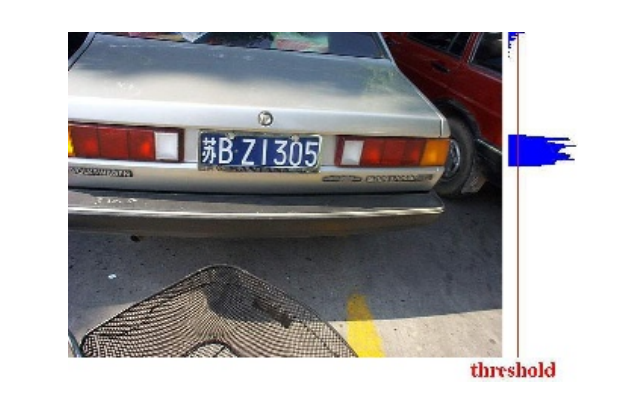
\includegraphics[width=\linewidth]{figures/shi_2005_1png.png}
    \caption{Localizarea zonei de interes generale folosind proiecții verticale}
  \end{subfigure}

  \vspace{1em}

  \begin{subfigure}[b]{0.4\linewidth}
    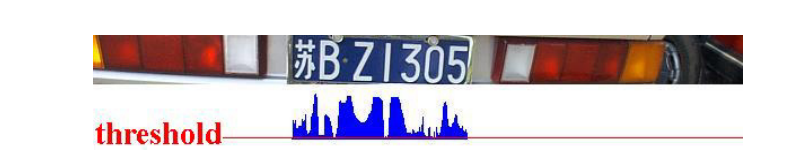
\includegraphics[width=\linewidth]{figures/shi_2005_2.png}
    \caption{Extragerea numărului de înmatriculare folosind proiecții verticale}
  \end{subfigure}
  \hfill
  \begin{subfigure}[b]{0.4\linewidth}
    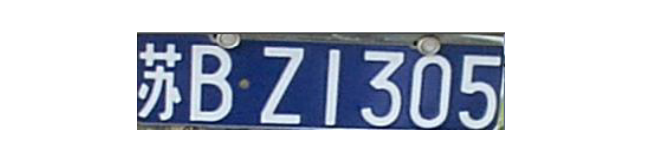
\includegraphics[width=\linewidth]{figures/shi_2005_3.png}
    \caption{Numărul de înmatriculare extras}
  \end{subfigure}
  \caption{Procesul de extracție al numărului de înmatriculare~\cite{shi2005automatic}}
\end{figure}

A doua lucrare~\cite{chang2004automatic} abordează plăcuțele din Taiwan, care utilizează patru culori distincte (alb, negru, roșu și verde). De această dată imaginea RGB este transformată efectiv în modelul HSI (Hue, Saturation, Intensity), pe baza căruia se construiește un detector de contururi cromatice. Spre deosebire de un detector de margini clasic, acesta reacționează doar la cele trei tipuri de tranziții întâlnite în interiorul plăcuței --- negru-alb, roșu-alb și verde-alb ---, ignorând restul contururilor din imagine. Pentru fiecare dintre hărțile de nuanță, saturație, intensitate și contur se calculează câte o hartă \emph{fuzzy}, ale cărei valori exprimă gradul în care fiecare pixel aparține unei plăcuțe. Cele patru hărți sunt apoi combinate printr-un agregator fuzzy în două etape, iar regiunile cu valori maxime locale și dimensiune suficientă sunt reținute drept candidați. Folosind exclusiv informația de localizare, metoda atinge o rată de succes de 97,9~\%, respectiv 93,7~\% pentru întregul sistem de recunoaștere.

Această categorie de metode prezintă atât avantaje, cât și limitări importante. Pe de o parte, atunci când contextul problemei garantează o paletă cromatică standardizată, ele oferă o acuratețe ridicată și un timp de execuție redus, datorită algoritmilor relativ simpli și ușor de optimizat. Pe de altă parte, ele nu generalizează la un spectru larg de formate, fiind dependente de un set restrâns de combinații de culori cunoscute \emph{a priori}; din acest motiv, lucrările menționate vizează țări precum China sau Taiwan, unde variațiile sunt limitate. În plus, performanța lor rămâne sensibilă la condițiile de iluminare și la degradarea cromatică a plăcuțelor reale.

\subsection{Metode bazate pe conturul obiectelor}
\indent\par
Această abordare are la bază presupunerea că în interiorul plăcuței există o densitate ridicată de linii verticale și orizontale care fac regiunea respectivă să iasă în evidență. Indiferent de abordarea ulterioară, fluxul de procesare începe întotdeauna de la transformarea imaginii în tonuri de gri. În fotografie și viziune pe calculator, o imagine în tonuri de gri este o imagine în care fiecare pixel este o nuanță de gri, unde valoarea fiecărei celule este un singur eșantion, ținând doar informația intensității. Această caracteristică a imaginilor în tonuri de gri reprezintă un factor important, deoarece în cadrul trecerilor, mai exact la marginile unui obiect apar întotdeauna diferențe mari de intensitate, cu atât mai mult în cadrul unui număr de înmatriculare unde trecerile sunt în general de la alb la negru, roșu la alb, verde la roșu, etc. Treceri bruște, clare și evidente într-o imagine convertită la alb-negru.

În~\cite{luo2009efficient} asupra imaginii convertite este aplicat operatorul Sobel pentru a extrage atât marginile verticale cât și cele orizontale. Operatorul Sobel constă în 2 kernel-uri specializate pentru detectarea liniilor convoluționate asupra întregii imagini pentru a produce un rezultat care evidențiază marginile obiectelor, trecerile bruște de la o intensitate la alta. Rezultatul intermediar generat de operatorul Sobel este binarizată folosind diferiți algoritmi de prag precum metoda histogramei, grad4 etc. Pentru o localizare robustă sunt aplicate imaginea \emph{skip} și imaginea integrală, prima având ca scop calcularea, pentru un dreptunghi de dimensiune predefinită, a distanței dintre pixelii albi și cei negri, iar imaginea integrală calculează pentru fiecare punct suma cumulativă a intensităților tuturor pixelilor aflați în regiunea superioară și stângă. Folosind această metodă, autorii au reușit să obțină o rată de localizare cu succes a numărului de înmatriculare de 99,95~\% cu un timp mediu de procesare de 47~\text{ms}.
\begin{figure}[h!]
  \centering
  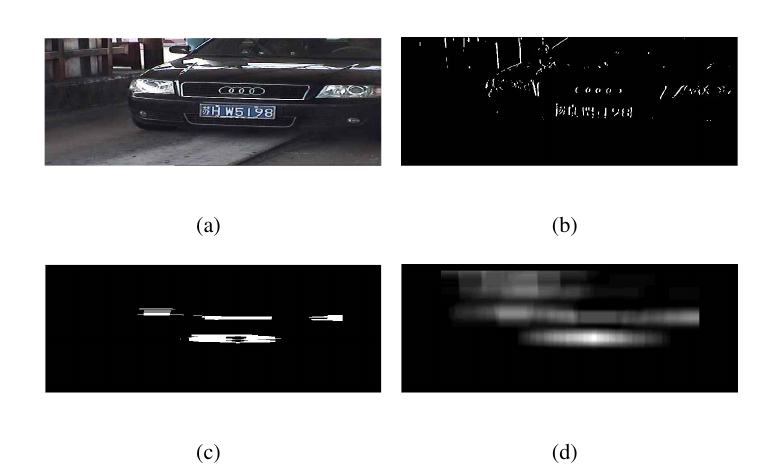
\includegraphics[width=0.6\linewidth]{figures/luo2209}
  \caption{(a) Imaginea RGB inițială, (b) Imaginea binară a marginilor, (c) Imaginea \emph{skip}, (d) Imaginea integrală~\cite{luo2009efficient}}
\end{figure}

Similar cu~\cite{luo2009efficient},~\cite{morph_operations} utilizează operatorul Sobel ca componentă primară pentru extragerea marginilor și a contururilor, totuși deosebirile apar încă din etapa de pre-procesare a imaginii (etapa de pre-procesare este formată din întreaga suită de pași aplicată imaginii înainte ca algoritmul principal de detectare a contururilor să fie rulat).~\cite{morph_operations} se folosesc de filtrul median pentru a atenua zgomotul imaginii. În viziunea pe calculator, atenuarea zgomotului presupune crearea unei funcții care capturează informațiile și tiparele imaginii lasând la o parte detaliile la scară redusă sau alte variații rapide de intensitate.

Pe lânga filtrarea mediană, pentru a asigura un rezultat robust, autorii definesc o mască de dimensiuni predefinite preluate din condiționarea problemei asupra căreia să continue cu urmatoarele etape ale procesului, respectiv operatorul Sobel, binarizarea imaginii și operația morfologică de deschidere. Aceasta din urmă constă în aplicarea consecutivă a două transformări fundamentale morfologice: eroziune și dilatare.

Operația de eroziune are rolul de a diminua obiectele din prim-plan și de a elimina structurile izolate care nu aparțin plăcuței. Aceasta presupune aplicarea unui kernel asupra întregii imagini, pixelul central fiind setat ca alb dacă toți pixelii acoperiți de kernel sunt la rândul lor albi. Operația de dilatare reprezintă opusul celei de eroziune, este formată din același algoritm, însă structura sa decizională transformă pixelul evaluat în „alb” dacă cel puțin un pixel acoperit de elementul structurant este activ.

\begin{figure}[h!]
  \centering
  \begin{subfigure}[b]{0.3\linewidth}
    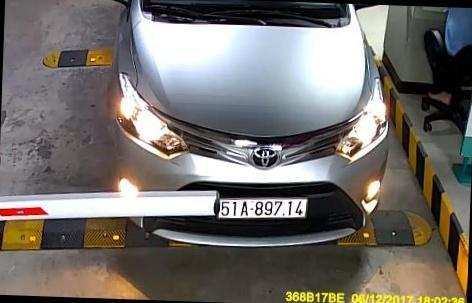
\includegraphics[width=\linewidth]{figures/input.jpg}
    \caption{Imagine de intrare}
  \end{subfigure}
  \begin{subfigure}[b]{0.3\linewidth}
    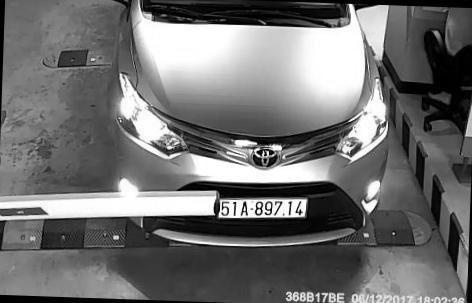
\includegraphics[width=\linewidth]{figures/greyscale.jpg}
    \caption{Imaginea în tonuri de gri}
  \end{subfigure}
  \begin{subfigure}[b]{0.3\linewidth}
    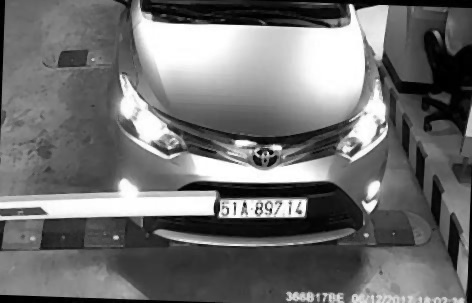
\includegraphics[width=\linewidth]{figures/median.jpg}
    \caption{Imaginea filtrată folosind filtrul median}
  \end{subfigure}
  \begin{subfigure}[b]{0.3\linewidth}
    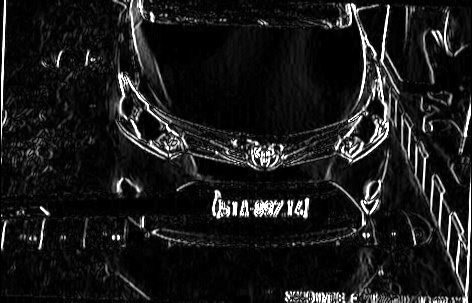
\includegraphics[width=\linewidth]{figures/sobel.jpg}
    \caption{Imaginea Sobel}
  \end{subfigure}
  \begin{subfigure}[b]{0.3\linewidth}
    
\includegraphics[width=\linewidth]{figures/open_image.jpg}
    \caption{Imaginea deschisă}
  \end{subfigure}
\end{figure}

Deși Sobel oferă rezultate bune, costul său din punct de vedere computațional a motivat autorii lucrării~\cite{VEDA} să dezvolte un nou algoritm pentru detectarea marginilor verticale. Metoda propusă omite în totalitate marginile orizontale din cadrul unei imagini, axându-se strict pe cele verticale. Această decizie a fost fundamentată pe observația că marginile orizontale pot cauza diferite elemente din compoziția mașinii precum grilajul să fie identificate în mod eronat drept numere de înmatriculare.

Fluxul de procesare propus în~\cite{VEDA} diferă față de cele menționate anterior. Inițial, asupra imaginii greyscale îî este aplicat un algoritm de binarizare cu prag adaptiv.

Acesta este urmat de ULEA (Unwanted Line Elimination Algorithm), un procedeu specializat de eliminare a artefactelor generate de către binarizare și a liniilor verticale nedorite de o lățime predefinită.

În final este aplicat VEDA, propus ca înlocuitor al operatorului Sobel de către autori. Această metodă constă în convoluționarea unui kernel de $2\times4$ asupra întregii imagini și o structură decizională care selectează un pixel ca fiind activ sau inactiv pe baza unor reguli logice în locul operațiilor clasice de convoluție.

Prin renunțarea la procesarea liniilor orizontale și optimizarea mecanismului de detecție, algoritmul propus are o viteză medie de rulare de 15~\text{ms}, o îmbunătățire semnificativă în comparație cu operatorul Sobel, care atinge o viteză medie de 130~\text{ms}.

\begin{figure}[h!]
  \centering
  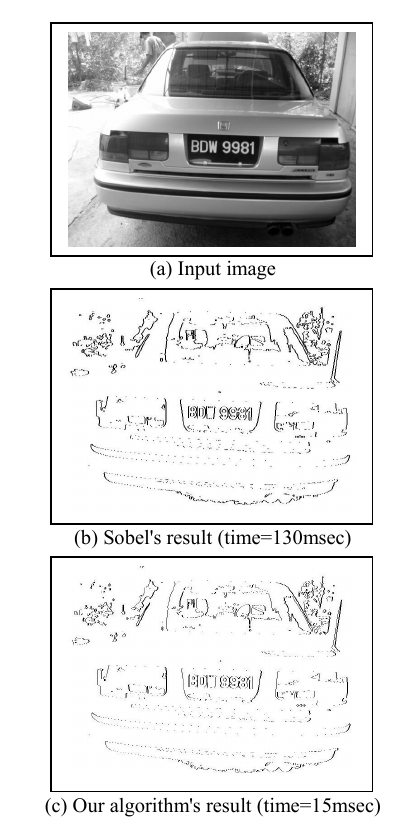
\includegraphics[width=0.3\linewidth]{figures/veda.png}
  \caption{Comparație între rezultatele generate de Sobel și VEDA~\cite{VEDA}}
\end{figure}

Datorită faptului că~\cite{luo2009efficient},~\cite{morph_operations},~\cite{VEDA} folosesc drept componentă principală operatorul Sobel, respectiv VEDA, aceste abordări sunt capabile să localizeze plăcuțe conținând numere de înmatriculare aflate în imagine la o înclinație de până la 15~\textdegree. Pentru a combate acest lucru, în~\cite{HoughTransformation} este folosit operatorul Hough drept selector principal.

Spre deosebire de operatorii de gradient (Sobel sau VEDA), care se bazează pe analiza locală a pixelilor, transformarea Hough reprezintă o tehnică de extracție a caracteristicilor utilizată pentru a identifica forme geometrice prin procesul de votare într-un spațiu al parametrilor. În contextul localizării numerelor de înmatriculare, aceasta este utilizată preponderent pentru detecția liniilor drepte care definesc conturul dreptunghiular al plăcuței.

Principiul fundamental constă în maparea fiecărui punct de margine $(x, y)$ din spațiul imaginii în spațiul polar $(\rho, \theta)$, utilizând ecuația:
$$\rho = x \cos(\theta) + y \sin(\theta)$$unde $\rho$ reprezintă distanța perpendiculară de la origine la dreaptă, iar $\theta$ este unghiul dintre axa $x$ și această perpendiculară.

Implementarea transformatii Hough în detrimentul implementării operatorului Sobel sau VEDA aduce anumite avantaje din punct de vedere al fiabilității sistemului, acesta fiind capabil sa localizeze în mod corect plăcuțe de înmatriculare înclinate la 30~\textdegree comparat cu 15~\textdegree. De asemenea, transformarea Hough nu este atât de sensibilă la variațiile de intensitate ale imaginii, astfel că o imagine de calitate nu este imperios necesară.

Totuși, performanța sporită vine cu un cost de complexitate computațională ridicat. Deoarece procesul de votare trebuie efectuat pentru fiecare pixel de margine și pentru o gamă largă de unghiuri, consumul de memorie (pentru matricea acumulator) și timpul de procesare sunt semnificativ mai mari față de un operator de convoluție simplu precum Sobel. Din acest motiv, în sistemele de timp real, transformarea Hough este adesea aplicată pe o regiune de interes (ROI) restrânsă sau este precedată de o etapă de binarizare agresivă pentru a reduce numărul de pixeli procesați.

\subsection{Metode bazate pe textura obiectelor}
\indent\par
Metodele bazate pe textură pornesc de la presupunerea că în interiorul numerelor de înmatriculare prezența caracterelor oferă o textură specifică și ușor diferențiabilă în comparație cu fundalul/ restul elementelor prezente în imagine.

În literatura de specialitate, există multiple abordări ale acestei categorii de metode,~\cite{bremananth2005robust},~\cite{anagnostopoulos2006license}, care se diferențiază prin modul în care este descrisă textura caracterelor și prin tehnica folosită pentru a evidenția regiunile cu densitate ridicată de tranziții.

În~\cite{bremananth2005robust} autorii aleg drept caracteristică definitorie a texturii densitatea de linii verticale prezente în cadrul numărului de înmatriculare. Aceștia propun un sistem al cărui prim pas este scăderea cromatică (\emph{color subtraction}), un algoritm ce primește ca parametri de intrare imaginea achiziționată anterior și o listă de elemente dintr-unul dintre modelele cromatice posibile; acest algoritm va păstra activi din imagine doar pixelii ale căror valori apar în lista primită drept parametru de intrare, iar pe restul îi va dezactiva. Următorul pas este aplicarea operatorului Sobel pentru a evidenția liniile verticale. În continuare va fi construită o hartă de densitate ponderată (\emph{weight-based density map}) folosind următorul algoritm de asignare a greutăților, în care creșterea, respectiv descreșterea unei greutăți asignate este direct proporțională:
\begin{align}
  W_{t_{\text{decr}}} &\propto (i - p) \\
  W_{t_{\text{decr}}} &\propto \gamma \\
  W_{t_{\text{decr}}} &= \partial\,\gamma\,(p - i) \\
  W_t &= \sum_{i=0}^{n} t_w \left( W_t + (px_i)\gamma + (1 - px_i)\big(\partial\gamma(p - i)\big) \right) \\
  t_w &= \frac{W_t - |W_t|}{-2W_t}\,\beta + \frac{W_t + |W_t|}{2W_t}
\end{align}
unde $\partial$ este constanta de decădere (\emph{decay constant}), $\gamma$ este factorul de incrementare a greutății, $\beta$ greutatea inițială, $n$ numărul de puncte de coordonate, $i$ coordonata muchiei curente, $p$ coordonata muchiei anterioare, iar $W_t$ valoarea greutății.

După finalizarea construcției hărții de densitate putem identifica posibilele regiuni în care apare un număr de înmatriculare.

Spre deosebire de~\cite{bremananth2005robust}, care descrie textura prin densitatea liniilor verticale, în~\cite{anagnostopoulos2006license} autorii pornesc de la ideea că plăcuța poate fi privită ca o regiune în care textura imaginii prezintă o „neregularitate'' locală pronunțată, mai exact treceri bruște și dese între caracterele întunecate și fundalul deschis. Pentru a evidenția aceste zone, ei propun o tehnică de segmentare adaptivă numită SCW (Sliding Concentric Windows), care nu măsoară direct contururile, ci variația statistică a intensităților dintr-o vecinătate.

Metoda se bazează pe utilizarea a două ferestre dreptunghiulare concentrice, una interioară $A$ de dimensiune $(2X_1) \times (2Y_1)$ și una exterioară $B$ de dimensiune $(2X_2) \times (2Y_2)$, care parcurg împreună întreaga imagine, pixel cu pixel, pornind din colțul stânga-sus. Pentru fiecare poziție se calculează în cele două ferestre câte o măsură statistică $M$ (media sau deviația standard a intensităților), iar pixelul central este clasificat în funcție de raportul dintre cele două măsuri:
$$I_{\text{AND}}(x, y) = \begin{cases} 0, & \text{dacă } \dfrac{M_B}{M_A} \leq T \\[2mm] 1, & \text{dacă } \dfrac{M_B}{M_A} > T \end{cases}$$unde $T$ este un prag stabilit experimental. Atunci când raportul depășește pragul, vecinătatea pixelului prezintă o variație texturală suficient de mare pentru ca acesta să fie considerat parte a unei regiuni de interes. Parametrii $X_1, X_2, Y_1, Y_2$ se aleg astfel încât raportul de aspect al ferestrelor să fie apropiat de cel al obiectelor căutate (caracterele plăcuței).

Imaginea binară $I_{\text{AND}}$ obținută prin SCW este apoi combinată cu imaginea originală printr-o operație logică ȘI, rezultatul fiind binarizat cu ajutorul metodei de prag adaptiv Sauvola, în care pragul fiecărui pixel depinde de media și deviația standard locale dintr-o fereastră de dimensiune $b \times b$:
$$T(x, y) = m(x, y)\left[1 + k\left(\frac{\sigma(x, y)}{R} - 1\right)\right]$$Asupra imaginii binarizate se aplică o analiză a componentelor conexe (CCA), iar obiectele rezultate sunt filtrate pe baza unor criterii geometrice: raportul de aspect, orientarea (sub $35~\textdegree$) și numărul Euler. Acesta din urmă, definit ca diferența dintre numărul de obiecte și numărul de „găuri'' interioare, este folosit pe baza observației că o plăcuță validă conține cel puțin patru caractere, deci minimum trei goluri ($E > 3$); regiunile care nu îndeplinesc aceste condiții sunt eliminate. Pentru a trata și plăcuțele cu fundal închis și caractere deschise, dacă nicio regiune candidată nu este găsită, imaginea este inversată și întregul proces reia.

Etapa de localizare este urmată de segmentarea caracterelor, realizată tot prin SCW aplicat regiunii decupate, și de recunoașterea propriu-zisă cu o rețea neuronală probabilistică (PNN) cu topologia $108\text{-}180\text{-}36$. Testat pe un set de 1334 de imagini din scene naturale, cu fundaluri și condiții de iluminare variate, sistemul a segmentat corect plăcuța în 96,5~\% din cazuri, recunoașterea întregii plăcuțe atingând 89,1~\%, respectiv o rată globală de succes de 86~\%.

\chapter{Segmentarea imaginii}\label{chap:segmentare}
Segmentarea imaginii joacă un rol crucial în sistemele ALPR. Procesul presupune divizarea imaginii într-un anumit număr de segmente informative, sau regiuni care sunt mai simple de studiat.

În literatura de specialitate, pentru a segmenta numărul de înmatriculare sunt propuse mai multe tehnici~\cite{SOAReview}:
\begin{itemize}
        \item{Analiza conectivității pixelilor~\cite{kanayama1991development}}
        \item{Analiza proiecțiilor}
        \item{Utilizarea informațiilor apriori privind aspectul caracterelor}
        \item{Analiza conturului caracterelor}
\end{itemize}

\subsection{Conectivitatea pixelilor}
Această abordare presupune binarizarea regiunii de interes extrase de modulul anterior, urmată de analiza componentelor conexe (CCA) și de aplicarea unei structuri decizionale pentru filtrarea regiunilor identificare de CCA. Selecția se bazează în principal pe criterii precum similitudinea dimensiunilor și a proporțiilor zonelor identificate de CCA.

Principalul dezavantaj al acestei metode este sensibilitatea la rotație, selecția fiind realizată pe baza uniformității geometrice a regiunilor, numerele de înmatriculare rotite sau înclinate parțial sunt adesea segmentate în mod incorect.

\subsection{Analiza proiecțiilor}
Contrastul ridicat dintre fundalul plăcuței și caractere face ca, în urma binarizării, cele două să fie reprezentate prin valori opuse. Această proprietate stă la baza unei familii largi de metode de segmentare, care exploatează distribuția pixelilor prin combinarea analizei proiecțiilor verticale și orizontale.

O proiecție se obține prin construirea unei histograme a densității pixelilor activi de-a lungul uneia dintre cele două axe de coordonate, un pixel fiind considerat activ atunci când valoarea sa aparține unui interval predefinit. În cazul, frecvent întâlnit în literatura de specialitate, al imaginilor binarizate, pixelii activi iau una dintre valorile $0$ sau $255$.

Un exemplu reprezentativ este sistemul propus în~\cite{HoughTransformation}, în care extracția numărului de înmatriculare se bazează pe transformarea Hough pentru corectarea variațiilor de înclinare și rotație.

Segmentarea începe cu analiza proiecțiilor orizontale, prin care numărul de înmatriculare este divizat pe rânduri. Etapa este esențială pentru plăcuțele dispuse pe mai multe rânduri (precum cele ale motocicletelor), întrucât separarea pe rânduri normalizează proporțiile și dimensiunea relativă a caracterelor în raport cu sub-segmentul care le conține. În absența ei, o evaluare globală ar introduce discrepanțe majore: pe un singur rând un caracter ocupă aproximativ $85\%$ din înălțimea imaginii, în timp ce pe o plăcuță cu două rânduri ajunge la cel mult $50\%$.

După divizarea pe rânduri, proiecțiile verticale sunt utilizate pentru a determina pozițiile de început și de final ale fiecărui caracter. Segmentele astfel obținute sunt apoi filtrate printr-un set de constrângeri, menite să elimine elementele segmentate eronat drept caractere.

\begin{figure}[H]
  \centering
  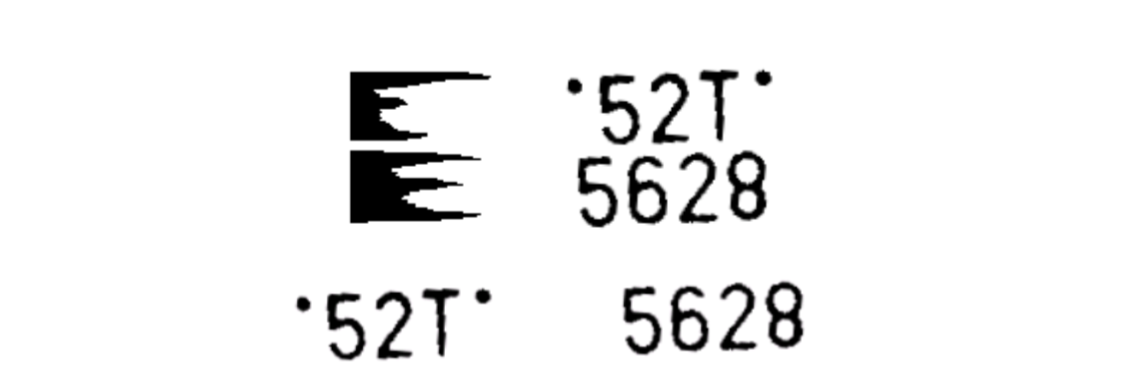
\includegraphics[width=\linewidth]{figures/hough_transformation_1png.png}
  \caption{Rezultatul divizării pe rânduri~\cite{HoughTransformation}}
\end{figure}

\begin{figure}[H]
  \centering
  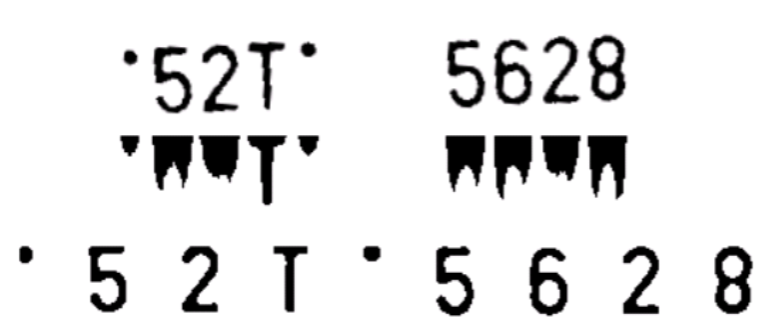
\includegraphics[width=\linewidth]{figures/hough_transformation_2.png}
  \caption{Rezultatul segmentării folosind proiecții verticale~\cite{HoughTransformation}}
  \label{fig:HoughSegmentation}
\end{figure}

\subsection{Utilizarea informațiilor apriori privind aspectul caracterelor}
Cunoștințe apriori în legătură cu aspectul caracterelor, font-ul, mărimea și proporțiile lor pot îmbunătăți în mod semnificativ procesul de segmentare.

În~\cite{sanyuan2004car} este propusă o abordare similară cu cea prezentată anterior în~\cite{HoughTransformation} în care numărul de înmatriculare este adus la o mărime și înclinare standard, iar etapa de segmentare este realizată folosind proiecții orizontale și verticale. Spre deosebire de metoda amintită în mod anterior, autorii se folosesc pe parcursul etapei de segmentare de o structură decizională care va ajuta la eliminarea rezultatelor fals-pozitive.

Particularitatea acestei abordări constă în combinarea informației furnizate de proiecția verticală cu cea obținută printr-o etapă preliminară de analiză a componentelor conexe (pre-extragerea zonelor conexe). Rolul acestei etape preliminare este de a atenua efectul zgomotului asupra proiecției: în prezența zgomotului, profilul de proiecție al imaginii binarizate prezintă punți (conexiuni) între caractere, care îngreunează separarea lor. Prin filtrarea prealabilă a zonelor conexe, numărul acestor conexiuni din profilul de proiecție se reduce semnificativ, motiv pentru care varianta astfel curățată este reținută pentru pașii următori, în detrimentul proiecției obținute direct din imaginea zgomotoasă.

Pe lângă atenuarea zgomotului, zonele conexe pre-extrase furnizează și informațiile apriori care stau la baza extragerii: lățimea caracterelor și poziția lor în cadrul plăcuței. Conform specificului plăcuțelor de înmatriculare avute în vedere, toate caracterele au aceeași lățime, care poate fi estimată direct din lățimea unei zone conexe deja izolate corect (de exemplu cifrele \textit{5} sau \textit{0}). Se definește poziția centrală a unui caracter ca fiind poziția orizontală a marginii sale stângi la care se adaugă jumătate din lățimea caracterului, iar distanța dintre pozițiile centrale a două caractere vecine se numește distanță între pozițiile centrale.

Geometria plăcuței impune o constrângere apriori suplimentară asupra acestor distanțe: ultimele cinci caractere au aceeași distanță între pozițiile centrale, în timp ce distanța $d_0$ dintre al doilea și al treilea caracter este mai mare decât distanța $d_1$ dintre celelalte caractere ($d_0 > d_1$). Experimental, cele două mărimi se află în relația
\begin{equation}
        d_0 = \lambda \cdot d_1, \qquad \lambda \in [1.2,\ 1.3].
\end{equation}

Folosind aceste cunoștințe apriori, procesul de extragere a caracterelor parcurge următorii pași:
\begin{enumerate}
        \item Din zona conexă pre-extrasă se determină intervalul vertical $h_0$ în care se află caracterele plăcuței.
        \item Tot din zona conexă pre-extrasă se obțin lățimea caracterului $w_1$ și pozițiile centrale ale caracterelor, ținând cont de constrângerile geometrice de mai sus (lățime constantă și distanțele $d_0$, $d_1$ dintre pozițiile centrale).
        \item Se scanează zonele conexe cuprinse în intervalul $h_0$ din imaginea plăcuței, integrând informația de poziție furnizată de proiecție; în funcție de rezultat se realizează fie combinarea mai multor zone într-un singur caracter, fie divizarea unei zone care înglobează mai multe caractere.
        \item Se furnizează rezultatul extragerii, care conține pozițiile caracterelor, acestea putând fi astfel izolate cu precizie.
\end{enumerate}

Acest proces adițional de selecție a regiunilor candidat sporește întreaga fiabilitate a sistemului deoarece elementele plăcuței care nu aparțin în-sine de numărul de înmatriculare precum șuruburile de fixare extrase în fig.~\ref{fig:HoughSegmentation} nu vor fi considerate mai departe drept zone de interes.

\subsection{Analiza conturului caracterelor}
O altă abordare are la bază detecția contururilor caracterelor. Pentru aceasta, în~\cite{capar2006concurrent} este propus un proces compus din doi pași, fundamentat pe tehnici de segmentare ce utilizează metoda \textit{Fast Marching} ghidată de formă (shape-driven).

Metoda \textit{Fast Marching}, introdusă de Sethian~\cite{sethian1996fastmarching}, este un algoritm numeric folosit pentru a urmări evoluția unui front (a unei curbe) care se propagă monoton într-o singură direcție, dinspre o regiune inițială către exterior. Algoritmul este o particularizare a metodelor de tip \textit{level-set}, în care viteza de propagare este strict pozitivă, astfel încât odată ce frontul a depășit un punct nu se mai poate întoarce.

Din punct de vedere matematic, metoda calculează, pentru fiecare punct $x$ al imaginii, momentul de timp $T(x)$ la care frontul ajunge în acel punct. Această mărime este soluția ecuației eikonale:
\begin{equation}
        \lvert \nabla T(x) \rvert \, F(x) = 1,
\end{equation}
unde $F(x)$ reprezintă funcția de viteză, care determină cât de rapid avansează frontul în fiecare punct. În aplicațiile de segmentare, funcția de viteză este derivată din informația din imagine (de regulă din magnitudinea gradientului): frontul se deplasează rapid în zonele omogene și încetinește, oprindu-se, în apropierea muchiilor, unde gradientul este mare. În acest fel, contururile obiectelor sunt delimitate în mod natural de zonele în care frontul stagnează.

Particularitatea abordării din~\cite{capar2006concurrent} constă în ghidarea propagării frontului nu doar de informația de contur, ci și de modele statistice ale formei caracterelor (\textit{shape-driven}). Funcția de viteză este astfel construită încât să integreze cunoștințe apriori despre forma caracterelor, permițând curbei să se oprească în dreptul muchiilor reale ale obiectelor și, în același timp, să inspecteze gradul de similaritate dintre conturul obținut și formele caracterelor cunoscute. Procesul realizează concomitent segmentarea și recunoașterea: pe parcursul evoluției frontului sunt determinate atât pozițiile delimitatoare ale fiecărui caracter, cât și eticheta (clasa) caracterului corespunzător, eliminând necesitatea unei etape separate de recunoaștere.

\chapter{Recunoașterea caracterelor}~\label{chap:recunoastere}
Ultima etapă, aceasta are ca scop identificarea și recunoașterea caracterelor prezente în regiunile selectate în etapa de segmentare.

General vorbind, pentru a atinge acest scop există două variante

\section{Potrivire de șabloane}
Această abordare, cunoscută sub denumirea de template matching, reprezintă metoda clasică de recunoaștere a caracterelor prin compararea directă a pixelilor. Procesul presupune existența unei baze de date cu șabloane (matrice) predefinite pentru fiecare caracter (litere și cifre), care sunt comparate succesiv cu regiunea segmentată până la identificarea celei mai bune potriviri.

Deși este eficientă din punct de vedere computațional datorită simplității algoritmice, această tehnică prezintă limitări severe în scenarii reale. Ea este aplicabilă cu succes doar atunci când caracterele extrase au dimensiuni, fonturi și grosimi constante, fiind extrem de sensibilă la variații geometrice.

Pentru a introduce un grad de robustețe și pentru a atenua sensibilitatea la zgomot sau mici distorsiuni, în locul unei suprapuneri binare perfecte, se utilizează algoritmi bazați pe calcularea distanțelor matematice între vectorii de trăsături: distanța Hamming~\cite{sarfraz2003saudi}, valoarea Jaccard~\cite{lee1994automatic}.

În mod concret,~\cite{sarfraz2003saudi} prezintă un sistem de recunoaștere a caracterelor format din două etape: normalizarea caracterelor și potrivirea șabloanelor. Prima etapă presupune aducerea regiunilor de interes extrase în etapa anterioară la o dimensiune standard de $40\times40$ prin intermediul unei transformări afine care mapează pixelii din imaginea originală la cei ai regiunii determinate anterior.

\begin{figure}[H]
  \centering
  \begin{subfigure}[b]{0.35\linewidth}
    \centering
    
\includegraphics[width=\linewidth]{figures/2003arabia_1.png}
    \caption{}
    \label{fig:2003arabia_a}
  \end{subfigure}
  \hspace{0.05\linewidth}
  \begin{subfigure}[b]{0.35\linewidth}
    \centering
    
\includegraphics[width=\linewidth]{figures/2003arabia_2.png}
    \caption{}
    \label{fig:2003arabia_b}
  \end{subfigure}
  \caption{ (a) Caracterul original, (b) Caracterul normalizat la o dimensiune standard de $40\times40$~\cite{sarfraz2003saudi}.}
  \label{fig:2003arabia}
\end{figure}

Pentru etapa de potrivire a șabloanelor, precum am menționat anterior, autorii se folosesc de distanța Hamming pentru a determina cel mai apropiat caracter. Formula acestei distanțe este descrisă de Ecuația 4.1.

\begin{equation}
  \begin{split}
    & \sum_{i=1}^{\text{nrows}} \sum_{j=1}^{\text{ncols}} \text{mismatch}_{i,j} \\
    & \text{mismatch}_{i,j} =
      \begin{cases}
        1, & \text{if } \text{original}_{i,j} \neq \text{extracted}_{i,j} \\
        0, & \text{if } \text{original}_{i,j} = \text{extracted}_{i,j}
      \end{cases}
  \end{split}
\end{equation}

\section{Clasificatori statistici}
Această metodă valorifică avansurile recente din domeniul inteligenței artificiale pentru a crea module de recunoaștere a caracterelor (OCR) robuste. Acestea prezintă o rezistența ridicată la variațiile de luminozitate, dimensiuni sau fonturi variate utilizate în creare numerelor de înmatriculare, etc. În literatura de specialitate, cele mai frecvent utilizate modele pentru această etapă a procesării imaginii sunt rețelele neuronale artificiale (ANN) și mașinile pe suport vectorial (SVM), ambele prezentând avantaje și limitări specifice.

S-ar putea spune că există o oarecare similitudine între SVM și ANN deoarece ambele își au rădăcinile în algoritmul perceptronului~\cite{rosenblatt1958perceptron}, însă abordările matematice care precedă acest algoritm diferă fundamental.

\section{Mașini pe suport vectorial}
Algoritmul ce stă la baza mașinilor pe suport vectorial reprezintă o generalizare a algoritmului ”portret generalizat” dezvoltat la începutul anilor 1960~\cite{vapnik1963pattern},~\cite{vapnik1964note}. Fundamentele matematice ale regresiei/ clasficării vectoriale sunt ancorate în învățarea statistică și teoria VC, care oferă o măsură a capacității de învățare a unui algoritm de învățare automată~\cite{vapnik2015uniform}.

Este important de menționat că algoritmul perceptronului funcționează prin actualizarea vectorului de greutăți w pornind de la o valoare inițială arbitrară, de regulă vectorul nul. Acesta este modificat prin adunarea exemplelor pozitive clasificate în mod eronat ca fiind negative, sau prin scăderea exemplelor negative clasificate ca fiind pozitive. Așadar, rezultatul final va fi întotdeauna o combinație liniară a punctelor din setul de antrenament.
\[ \mathbf{w} = \sum_{i=1}^{\ell} \alpha_i y_i \mathbf{x}_i, \]

Unde semnul ecuației este dat de clasificarea $y_i \in \{-1, 1\}$, iar valorile $\alpha_i$ sunt valori pozitive proporționale cu numărul de misclasificări făcute asupra punctului în timpul stagiului de antrenament. Punctele care au cauzat mai puține erori, vor avea un $\alpha_i$ mai mic, iar punctele dificile unul mai mare. Date fiind aceste valori, perceptronul poate fi rescris folosind următoarea formulă:
\[ h(\mathbf{x}) = \operatorname{sgn} \left( \sum_{j=1}^{\ell} \alpha_j y_j \langle \mathbf{x}_j \cdot \mathbf{x} \rangle + b \right) \] numită și forma duală a perceptronului.

Datorită acestei reprezentări duale, este posibilă utilizarea kernel trick-ului care ne permite maparea într-o dimensiune diferită a atributelor primite ca input. O astfel de mapare este benefică deoarece ne permite selectarea și rafinarea atributelor la un nivel mult mai granular. Cu ajutorul kernel trick-ului, algoritmul perceptronului în formă duală nu mai depinde de calcularea explicită a vectorului de greutăți în spațiul trăsăturilor, ci de evaluarea produsului scalar dintre vectorii de intrare mapați
$$ f(\mathbf{x}) = \text{sgn} \left( \sum_{i=1}^{\ell} \alpha_i y_i K(\mathbf{x}_i, \mathbf{x}) + b \right) $$
unde $K(\mathbf{x}_i, \mathbf{x})$ reprezintă funcția kernel, definită ca produsul scalar al funcțiilor de mapare $\phi(\mathbf{x})$ (sau $\theta(\mathbf{x})$).

\section{Teoria VC și clasificatori cu marjă maximală}
Spre deosebire de algoritmul perceptronului, care se oprește în momentul în care identifică un hiperplan care separă corect punctele setului de antrenament, fără a oferi nicio garanție asupra performanței pe date nevăzute, mașinile pe suport vectorial sunt fundamentate teoretic pe principiul minimizării riscului structural derivat din teoria Vapnik-Chervonenkis (VC)~\cite{vapnik2015uniform}.

Conceptul central al acestei teorii îl constituie dimensiunea VC, o măsură a capacității de exprimare a unei familii de funcții de clasificare. În mod formal, dimensiunea VC reprezintă cardinalitatea celui mai mare set de puncte care poate fi etichetat (pulverizat) în toate modurile binare posibile de către funcțiile clasei respective. O dimensiune VC ridicată indică un model cu o capacitate sporită de a se mula pe orice configurație a datelor, dar și un risc proporțional crescut de supra-învățare, deoarece marja garantată între eroarea empirică (pe setul de antrenament) și eroarea reală (așteptată pe distribuția datelor) crește odată cu dimensiunea VC. În consecință, controlul acestei dimensiuni reprezintă o cerință esențială pentru asigurarea capacității de generalizare a modelului.

În cazul particular al hiperplanelor în spațiul $\mathbb{R}^n$, dimensiunea VC este, în general, $n+1$. Totuși, dacă restrângem familia clasificatorilor la submulțimea hiperplanelor care separă datele cu o marjă $\gamma$ și presupunem că punctele de antrenament sunt incluse într-o sferă de rază $R$, atunci dimensiunea VC efectivă a clasei rezultate este mărginită superior de raportul $R^2/\gamma^2$~\cite{vapnik2015uniform},~\cite{svmIntroduction}. Această observație fundamentală oferă justificarea teoretică pentru abordarea adoptată de SVM: prin maximizarea marjei $\gamma$, se reduce implicit dimensiunea VC a familiei de funcții utilizate, ceea ce conduce la limite superioare mai stricte asupra erorii de generalizare, independent de dimensionalitatea spațiului trăsăturilor.

Formal, problema clasificatorului cu marjă maximală se reduce la rezolvarea problemei de optimizare convexă:
\[
\min_{\mathbf{w}, b} \frac{1}{2} \|\mathbf{w}\|^2 \quad \text{cu restricția} \quad y_i(\mathbf{w}^\top \mathbf{x}_i + b) \geq 1, \quad i = 1, \dots, \ell,
\]
unde minimizarea normei $\|\mathbf{w}\|$ este echivalentă cu maximizarea marjei $\gamma = 1/\|\mathbf{w}\|$. Această proprietate este deosebit de relevantă în contextul recunoașterii caracterelor de pe plăcuțele de înmatriculare, deoarece spațiile de trăsături utilizate (vectori obținuți prin caracteristici HOG, momente Zernike sau pixeli normalizați) sunt frecvent înalt dimensionale, iar capacitatea unui clasificator de a evita supra-învățarea într-un astfel de regim este critică.

Pentru a permite tratarea seturilor de date care nu sunt liniar separabile, formularea originală a fost extinsă prin introducerea variabilelor de relaxare $\xi_i$ și a parametrului de penalizare $C$~\cite{cortes1995support}, conducând la formularea cu marjă moale:
\[
\min_{\mathbf{w}, b, \xi} \frac{1}{2} \|\mathbf{w}\|^2 + C \sum_{i=1}^{\ell} \xi_i \quad \text{cu restricția} \quad y_i(\mathbf{w}^\top \mathbf{x}_i + b) \geq 1 - \xi_i, \quad \xi_i \geq 0.
\]
Parametrul $C$ controlează raportul dintre maximizarea marjei și tolerarea erorilor de clasificare, permițând astfel un compromis explicit între capacitatea modelului și riscul empiric. Combinat cu utilizarea funcțiilor kernel introduse prin~\cite{boser1992training}, acest cadru permite construirea unor clasificatori cu putere de discriminare ridicată, păstrând în același timp un control formal asupra capacității de generalizare.

\section{Rețele neuronale artificiale}
Rețelele neuronale artificiale (ANN) reprezintă cea de-a doua direcție majoră în recunoașterea caracterelor din cadrul plăcuțelor de înmatriculare. Spre deosebire de SVM, care își are fundamentul în teoria învățării statistice, ANN-urile sunt inspirate dintr-un model simplificat al activității neuronilor biologici și se bazează pe compunerea ierarhică a unităților elementare derivate din perceptronul lui Rosenblatt~\cite{rosenblatt1958perceptron}.

Perceptronul multistrat (MLP), constă într-un strat de intrare, unul sau mai multe straturi ascunse și un strat de ieșire. Fiecare neuron $j$ dintr-un strat efectuează o transformare afină asupra activărilor stratului precedent, urmată de aplicarea unei funcții de activare neliniare $\sigma$:
\[
a_j = \sigma\left( \sum_{i} w_{ji} x_i + b_j \right).
\]
Compoziția acestor transformări permite rețelei să construiască, în mod implicit, reprezentări ale datelor de complexitate crescândă. Justificarea teoretică pentru această abordare este oferită de teorema aproximării universale, care stabilește că o rețea cu un singur strat ascuns și un număr suficient de neuroni poate aproxima, cu precizie arbitrară, orice funcție continuă definită pe un domeniu compact~\cite{hornik1989multilayer}.

Antrenarea ANN-urilor este realizată prin algoritmul de retropropagare a erorii~\cite{rumelhart1986learning}, urmat de o actualizare iterativă a acestora prin metode bazate pe coborârea gradientului. În contextul recunoașterii caracterelor de pe plăcuțele de înmatriculare, intrarea este, în mod tipic, o imagine segmentată corespunzătoare unui singur caracter, normalizată la o rezoluție fixă, iar ieșirea reprezintă o distribuție de probabilitate peste setul de clase posibile (literele alfabetului și cifrele 0--9), obținută prin aplicarea funcției softmax.

Comparativ cu SVM, ANN-urile prezintă avantajul de a învăța automat reprezentări intermediare ale datelor, fără a necesita o etapă explicită de inginerie a trăsăturilor. Acest fapt este deosebit de util în prezența variațiilor de font, grosime a caracterelor sau ușoare deformări geometrice. Pe de altă parte, antrenarea ANN-urilor necesită seturi de date considerabil mai voluminoase, este sensibilă la inițializarea parametrilor și nu beneficiază de garanții de generalizare la fel de stricte precum cele derivate din teoria VC pentru SVM-urile cu marjă maximală.


\chapter{Implementarea sistemului IORA}\label{chap:implementare}
\indent\par
Sistemul propus în lucrarea de față, denumit IORA, a fost construit pornind de la o arhitectură modulară formată din trei componente cheie: modulul de preluare a datelor (\textit{Input Module}), fluxul de procesare (\textit{Processing Pipeline}) și modulul de logică a aplicației (\textit{Application Logic Module}). Pentru a oferi flexibilitate și a respecta principiile de proiectare extensibilă specifice conceptului de \textit{clean code}~\cite{codecomplete}, modulul de intrare și cel de logică a aplicației utilizează polimorfismul prin expunerea unor interfețe abstracte.

Această abordare decuplată permite diferitelor aplicații să integreze nucleul sistemului într-un mod elegant, implementând comportamente personalizate și adaptate la mediul de execuție, fără a modifica codul de bază. De exemplu, modulul de intrare poate fi extins pentru a prelua fluxuri video de la o cameră atașată mediului de execuție, fie prin intermediul \textit{socket-urilor}. În mod similar, modulul de logică a aplicației poate fi personalizat pentru a declanșa acțiuni specifice precum trimiterea unor notificări automate prin \textit{e-mail}, sau acționarea unor echipamente \textit{hardware}, în cazul unui sistem integrat.

În contrast, fluxul de procesare este încapsulat ca o unitate de execuție independentă și de sine stătătoare, neexpunând nicio interfață publică destinată extinderii structurale.

În continuare, acest capitol descrie arhitectura și tehnologiile utilizate în implementarea aplicației prezentate alături de o descriere tehnică a fiecărui modul.

\section{Arhitectura sistemului}
\indent\par
Sistemul IORA este organizat pe trei niveluri logice care corespund celor trei module introduse la începutul capitolului: nivelul de achiziție a datelor, nivelul de procesare și nivelul de logică a aplicației. Această stratificare urmărește o separare clară a responsabilităților, fiecare nivel comunicând cu cel adiacent exclusiv prin structuri de date simple, independente de bibliotecile externe folosite în implementare. Decuplarea astfel obținută permite ca un nivel să fie înlocuit sau extins fără a afecta restul sistemului.

\subsection{Diagrama de componente}
\indent\par
Diagrama de componente, prezentată în Figura~\ref{fig:componente}, surprinde cele trei module și fluxul de date dintre ele. Modulul de intrare expune interfața \texttt{ICaptureManager} și produce, indiferent de sursa fizică a datelor, obiecte de tip \texttt{Frame}. Aceste obiecte constituie singurul punct de contact dintre modulul de intrare și fluxul de procesare, eliminând orice dependență a nucleului de natura sursei de captură.

Fluxul de procesare consumă obiectul \texttt{Frame} și aplică, în mod secvențial, cele trei etape ale procesului de recunoaștere: localizarea plăcuței, segmentarea caracterelor și recunoașterea acestora. Rezultatul produs (șirul de caractere recunoscut, însoțit de metadatele asociate) este transmis mai departe către modulul de logică a aplicației, care decide acțiunea declanșată în funcție de contextul de execuție.

\begin{figure}[H]
  \centering
  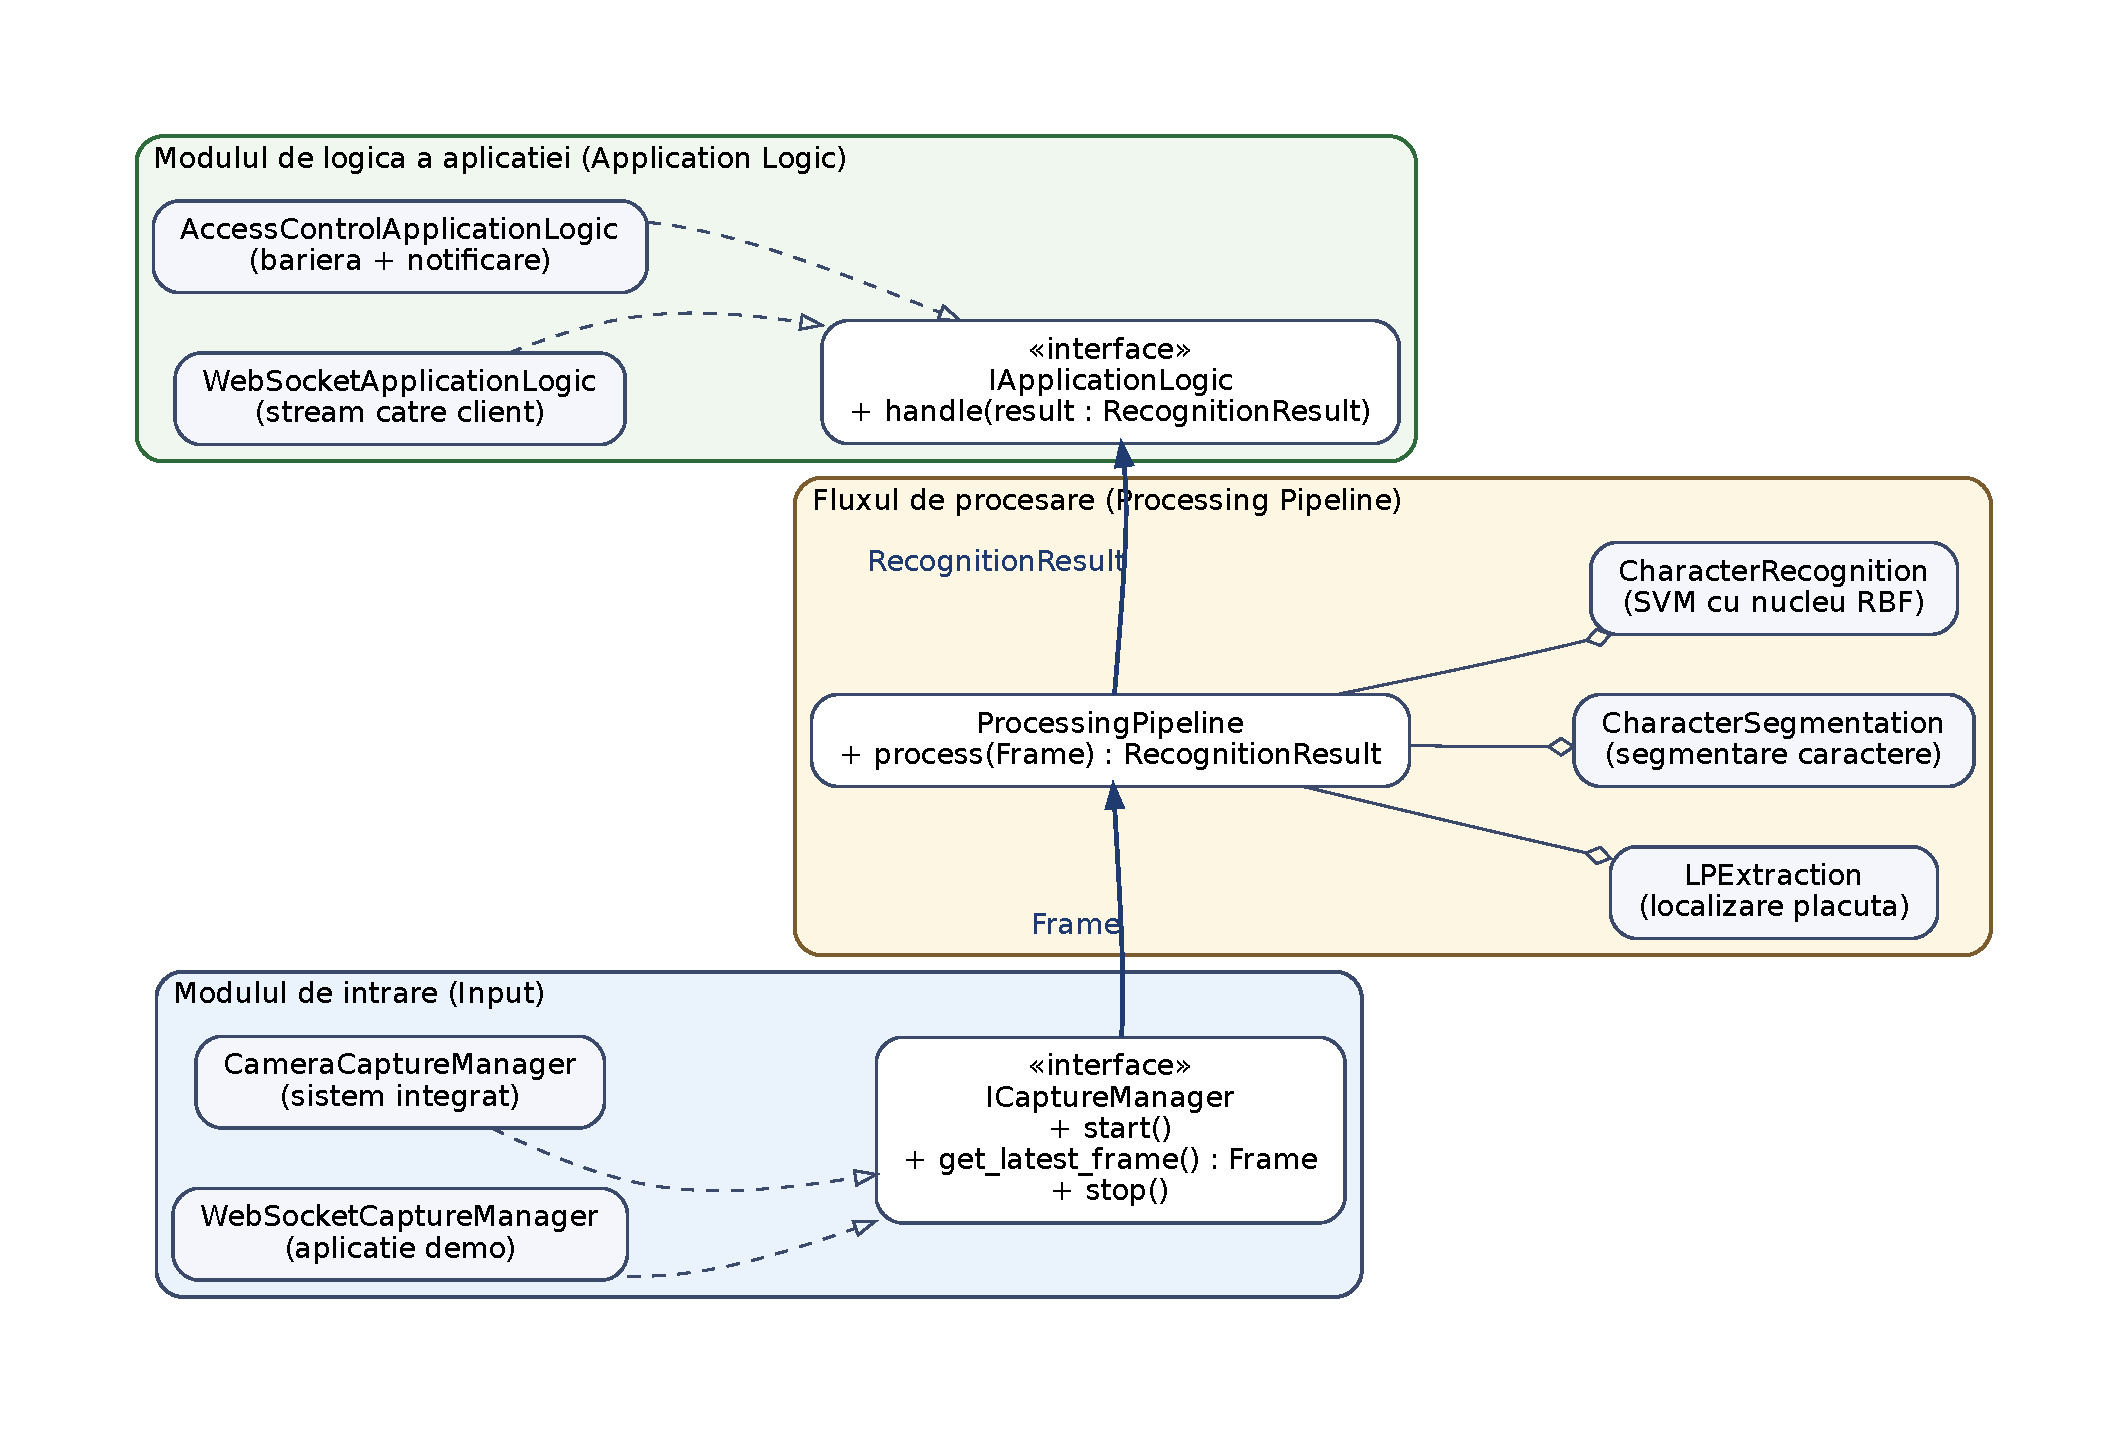
\includegraphics[width=0.9\linewidth]{figures/iora_componente.pdf}
  \caption{Diagrama de componente a sistemului IORA: modulele de intrare,
    procesare și logică a aplicației, împreună cu structurile de date
    \texttt{Frame} și \texttt{RecognitionResult} care le decuplează.}
  \label{fig:componente}
\end{figure}

\subsection{Actori și cazuri de utilizare}
\indent\par
În cadrul scenariului de utilizare vizat, sistemul interacționează cu mai mulți actori, atât umani, cât și automați. Actorul uman principal este operatorul, responsabil de configurarea și monitorizarea sistemului. Actorii automați sunt reprezentați de echipamentele și serviciile care consumă rezultatul recunoașterii: sistemul de barieră (acționat în urma unei recunoașteri valide) și serviciul de notificare (care transmite alerte, de exemplu prin \textit{e-mail}).

Principalele cazuri de utilizare sunt: monitorizarea fluxului video de la sursa de captură, citirea automată a numărului de înmatriculare dintr-un cadru și declanșarea unei acțiuni asociate (ridicarea barierei sau emiterea unei notificări) pe baza rezultatului recunoașterii. Pentru aplicația demonstrativă, se adaugă cazul de utilizare al transmiterii rezultatelor către un client extern prin intermediul unei conexiuni \textit{WebSocket}. Aceste cazuri de utilizare, împreună cu actorii implicați, sunt sintetizate în Figura~\ref{fig:usecase}.

\begin{figure}[H]
  \centering
  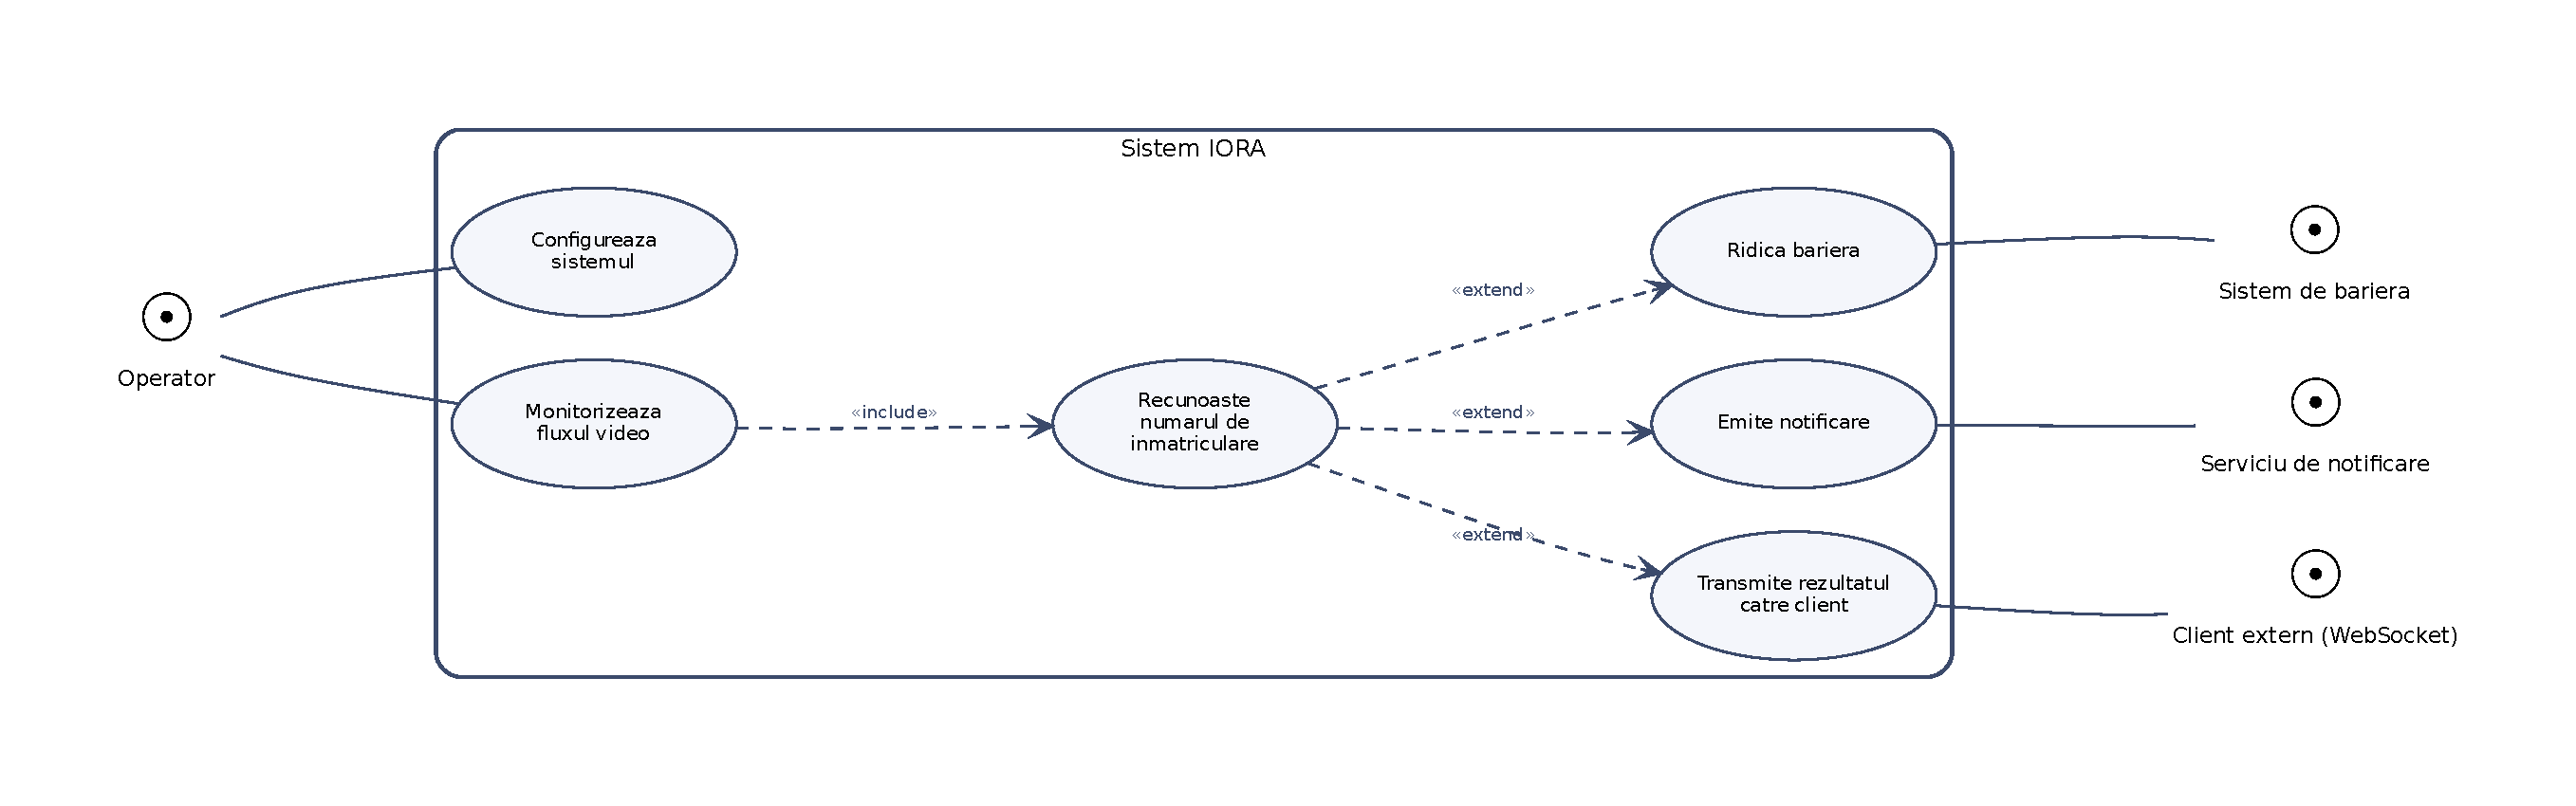
\includegraphics[width=\linewidth]{figures/iora_usecase.pdf}
  \caption{Diagrama cazurilor de utilizare a sistemului IORA, cu operatorul
    drept actor uman principal și sistemele consumatoare ale rezultatului
    recunoașterii drept actori automați.}
  \label{fig:usecase}
\end{figure}

\subsection{Diagrama de clase}
\indent\par
Diagrama de clase din figura~\ref{fig:clase} reflectă, la nivel structural, aceeași stratificare introdusă de diagrama de componente: interfețele \texttt{ICapture\-Manager} și \texttt{IApplication\-Logic} delimitează marginile extensibile ale sistemului, fiecare având două realizări concrete (una pentru sistemul integrat, una pentru aplicația demonstrativă), în timp ce nucleul de procesare este modelat prin clasa \texttt{ProcessingPipeline}, care agregă cele trei etape ale recunoașterii (\texttt{LPExtraction},\- \texttt{CharacterSegmentation},\- \texttt{CharacterRecognition}). Tipurile de date proprii \texttt{Frame} și \texttt{RecognitionResult} apar ca dependențe la marginile fluxului, marcând explicit decuplarea nucleului de detaliile de implementare ale surselor de captură și ale acțiunilor declanșate de aplicație.

\begin{figure}[H]
  \centering
  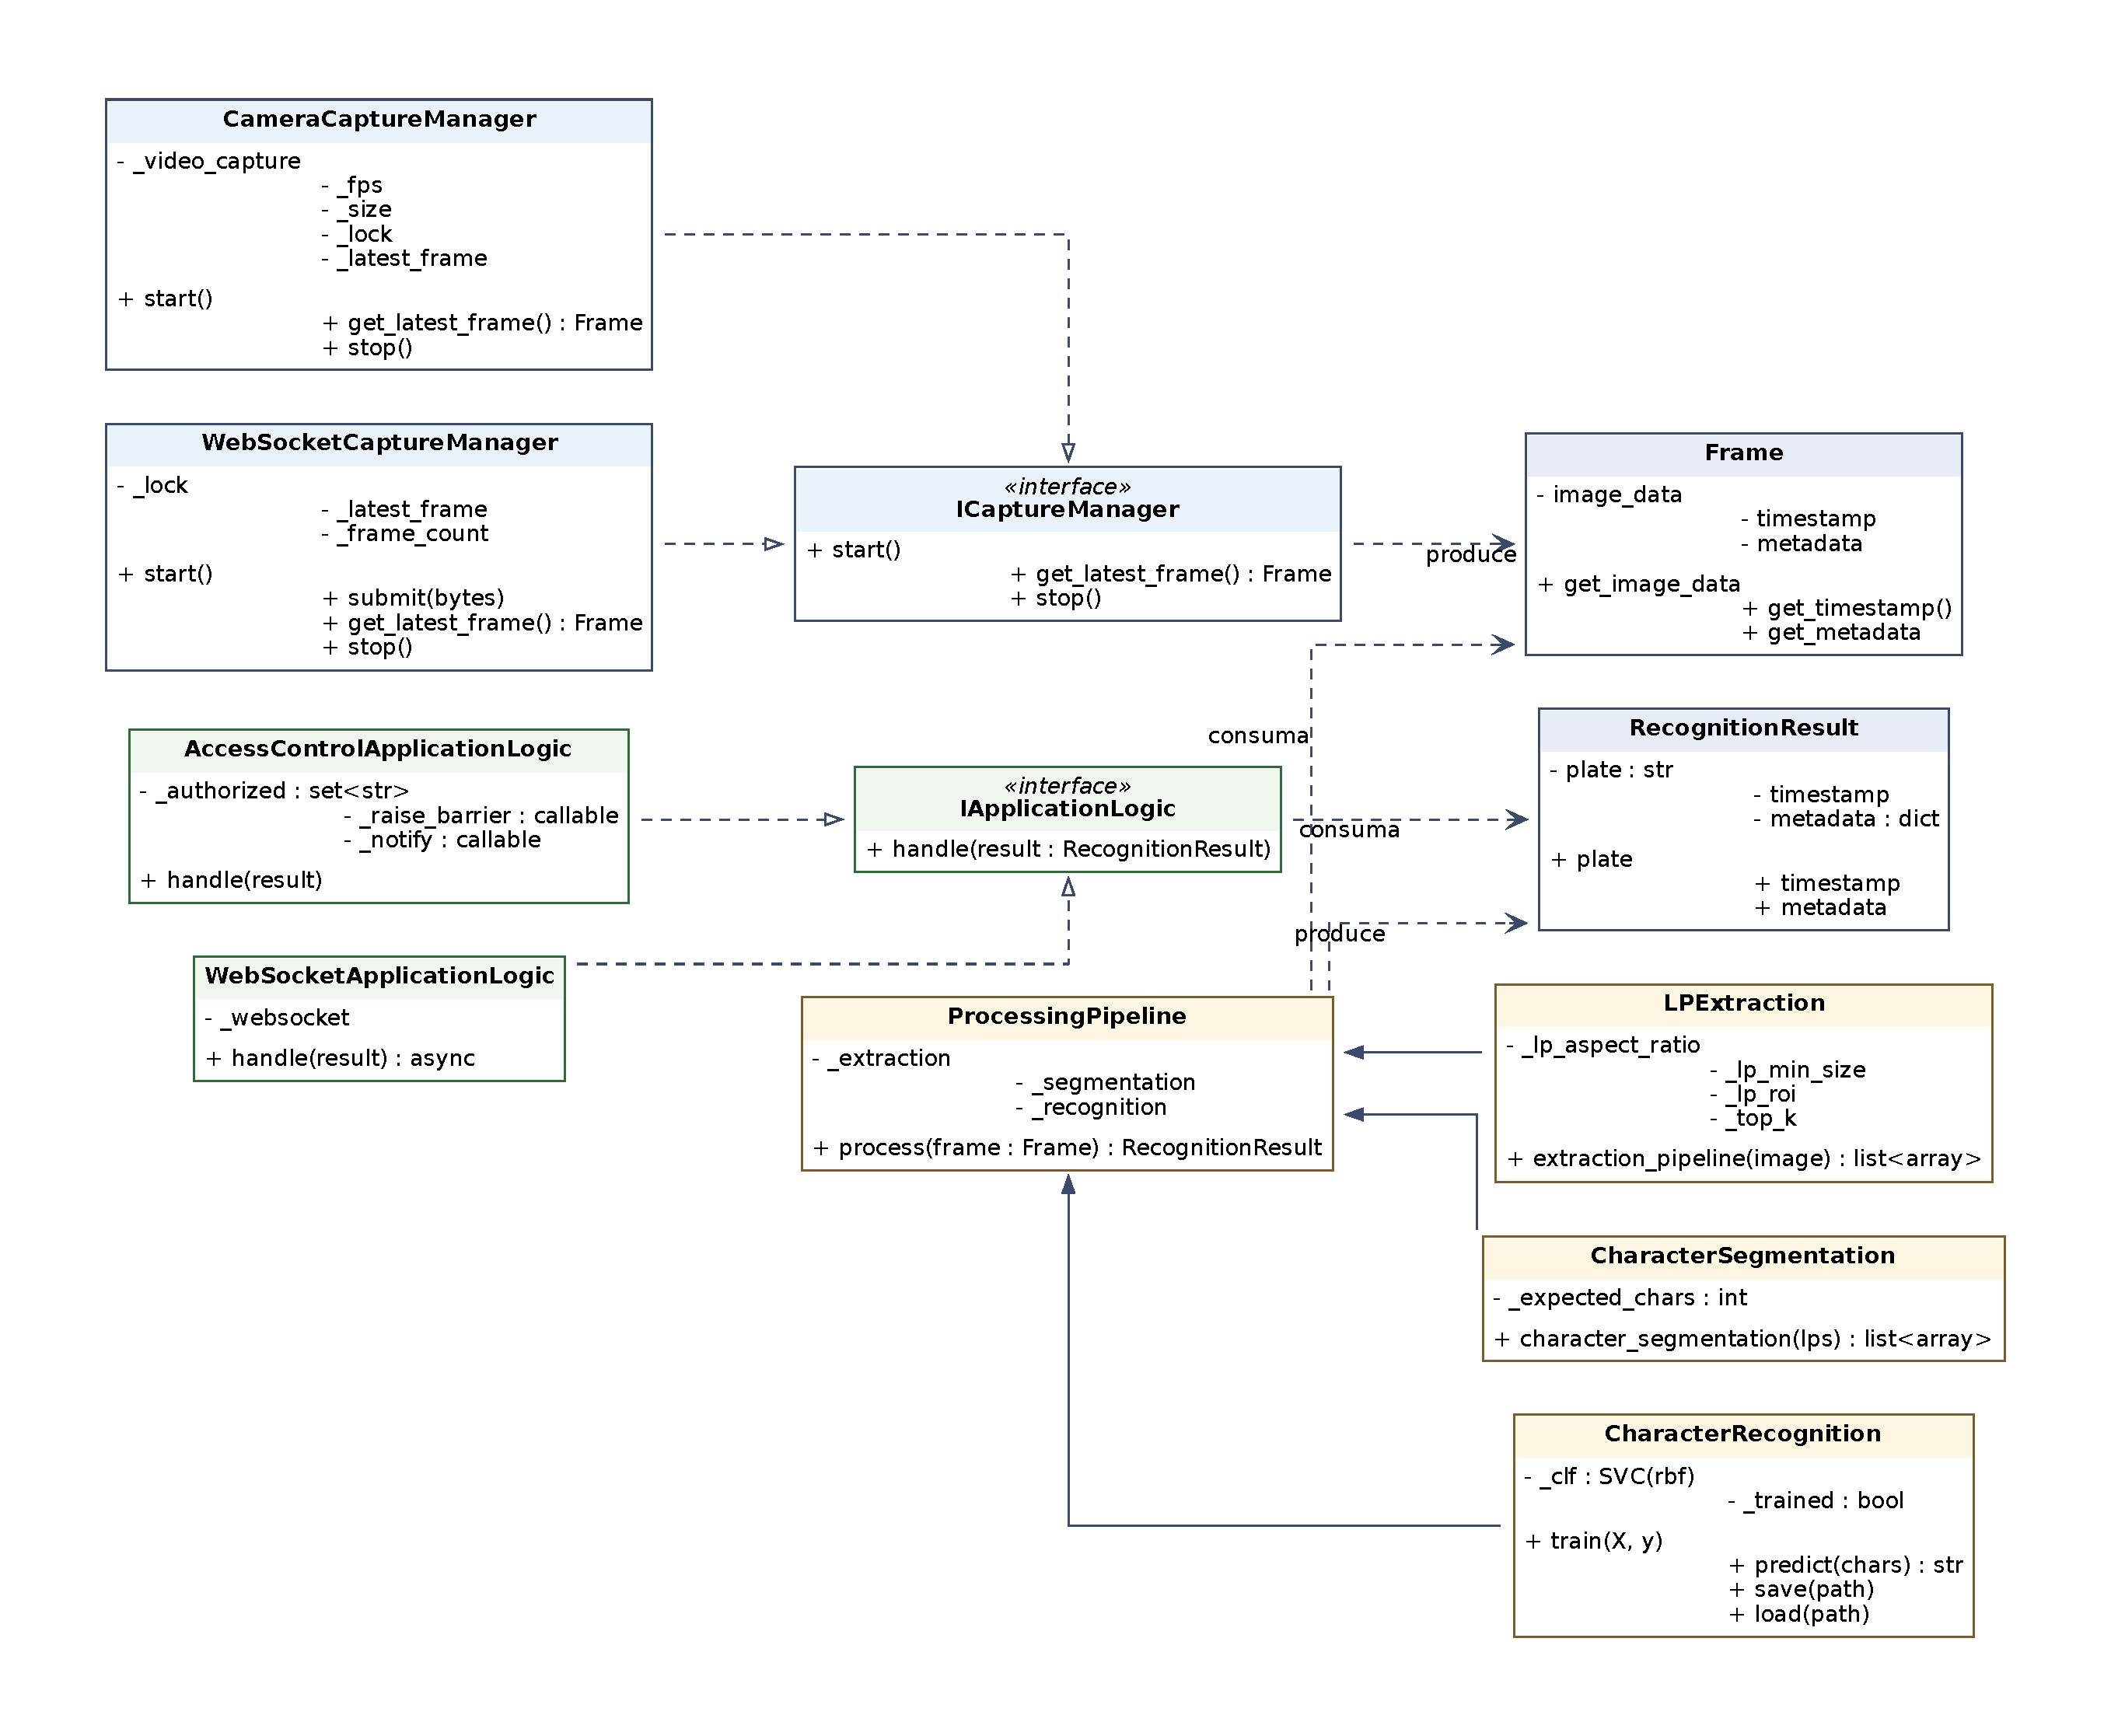
\includegraphics[width=\linewidth]{figures/iora_clase.pdf}
  \caption{Diagrama de clase a sistemului IORA: interfețele extensibile, realizările lor concrete și agregarea celor trei etape de procesare în \texttt{ProcessingPipeline}.}
  \label{fig:clase}
\end{figure}

\subsection{Decizii de proiectare}
\indent\par
Proiectarea bazată pe principiile arhitecturale menționate anterior sugerează natura componentelor: modulele de la margini interacționează direct cu mediul de execuție și sunt, prin urmare, cele mai susceptibile la variații, motiv pentru care comportamentul lor este abstractizat prin interfețe conform principiilor de \textit{clean code}~\cite{codecomplete}. În schimb, fluxul de procesare implementează un algoritm stabil, independent de context, care nu beneficiază de pe urma extensibilității.

O a doua decizie de proiectare vizează minimizarea dependențelor la nivelul nucleului și definirea unor tipuri de date proprii. Această alegere consolidează portabilitatea sistemului și permite adoptarea sa în contexte de rulare diferite, de la sisteme integrate cu resurse limitate până la servere care deservesc o aplicație web.

\section{Tehnologii}
\indent\par
Alegerea limbajului a fost făcută pe considerente practice, așadar întreg sistemul a fos implementat în Python 3.14.4 în detrimenul unui limbaj compilat precum C++. Această decizie a fost motivată de gradul ridicat de adopție a ecosistemului Python în cadrul sistemelelor integrate, precum și de flexibilitatea și viteza de dezvoltare specifice oferite de un limbaj dinamic. De asemenea, librăriile necesare implementării modului de procesare se bazează pe nuclee scrise în C.

Pentru a oferi o structură clară, tehnologiile utilizate au fost împărțite în două categorii: cele fundamentale, necesare dezvoltării nucleului și cele adiționale, specifice dezvolării aplicației finale.

\subsection{Nucleu}
\indent\par
Din punct de vedere tehnologic, implementarea nucleului se bazează pe un ecosistem minimalist de dependențe. Tehnologiile de bază utilizate sunt:
\begin{itemize}
  \item{OpenCV 4.13.0}
  \item{numpy 2.4.2}
  \item{scikit-learn 1.8.0}
  \item{matplotlib-base 3.10.9}
\end{itemize}

\subsection{Nivelul de aplicație}
\indent\par
După cum am menționat, dependențele necesare dezvoltării aplicației finale sunt opționale, acestea depinzând strict de contextul aplicației dorite. Pentru aplicația propusă, dependențele sunt:
\begin{itemize}
  \item{fastapi 0.135.4}
  \item{websockets 15.0.1}
\end{itemize}

\section{Detalii tehnice}
\indent\par
În cele ce urmează va fi prezentată o descriere detaliată a arhitecturii fiecărui modul, abordând aspecte precum interfețele de programare expuse, deciziile de proiectare și implementarea propriu-zisă.

Pentru modulele extensibile, se va realiza o paralelă între implementarea în cadrul unui sistem integrat și implementarea concretă realizată în cadrul aplicației demonstrate.

\subsection{Modulul de intrare}
\indent\par
Achiziția datelor de intrare reprezintă punctul de plecare al sistemului. Acest modul are rolul exclusiv de a prelua informația brută și de a o expune către fluxul de procesare. În continuare vor fi prezentate elementele atât abstracte cât și concrete ale acestei componente.

\subsubsection{Interfața ICaptureManager}
\indent\par
Interfața \texttt{ICaptureManager} este definită prin trei metode esențiale. Primele două, \texttt{start} și \texttt{stop}, gestionează ciclul de viață al sistemului de captură, ocupându-se de inițializarea și, respectiv, de eliberarea resurselor asociate acestuia. Cea de-a treia metodă, \texttt{get\_latest\_frame}, returnează cel mai recent cadru preluat, încapsulat într-un obiect de tip \texttt{Frame}.
\begin{verbatim}
    def start(self) -> None:
        pass

    def get_latest_frame(self) -> Frame:
        pass

    def stop(self) -> None:
        pass
\end{verbatim}

\subsubsection{Sistem integrat}
\indent\par
Pentru scenariul rulării pe un sistem integrat, a fost realizată o implementare exemplificativă, clasa \texttt{CameraCaptureManager}, responsabilă de preluarea cadrelor de la o cameră conectată direct la dispozitiv.

Implementarea se bazează pe biblioteca OpenCV pentru a media interacțiunea cu subsistemul de captură video al sistemului de operare. Identificarea sursei fizice se realizează prin intermediul indexului de dispozitiv asociat camerei, transmis ca parametru constructorului clasei.

Pe lângă indexul de dispozitiv, clasa expune următoarele atribute private:
\begin{itemize}
  \item{\texttt{\_video\_capture} - obiectul OpenCV prin care se realizează comunicarea cu camera;}
  \item{\texttt{\_fps} - numărul de cadre pe secundă raportat de dispozitiv;}
  \item{\texttt{\_size} - rezoluția cadrelor preluate, dedusă din primele cadre citite;}
  \item{\texttt{\_lock} - obiect necesar pentru sincronizarea accesului la cel mai recent cadru.}
\end{itemize}

Metoda \texttt{get\_latest\_frame} a fost proiectat astfel încât să returneze întotdeauna cel mai recent cadru disponibil. Această cerință este esențială într-un context de procesare în timp real: întrucât bibliotecile de captură mențin o memorie internă, citirea secvențială a cadrelor ar introduce o latență cumulativă, returnând cadre deja învechite. Pentru a evita acest fenomen, un fir de execuție (\textit{thread}) dedicat preia continuu cadrele de la cameră, păstrând disponibil doar cel mai recent dintre acestea. Accesul concurent la resursa partajată este sincronizat printr-un mecanism de tip \textit{lock}.

\subsubsection{Aplicație demonstrativă}
\indent\par
În cadrul aplicației demonstrative, sursa de captură nu este o cameră atașată direct dispozitivului, ci un flux video transmis în timp real (\textit{live-feed}) printr-o conexiune \textit{WebSocket}. Această implementare menține o conexiune persistentă prin care cadrele sosesc continuu de la un client extern, le decodează și le încapsulează în același obiect \texttt{Frame}. La fel ca în cazul implementării pentru sistemul integrat, doar cel mai recent cadru recepționat este păstrat disponibil, evitând acumularea unei latențe în contextul procesării în timp real.

\subsection{Fluxul de procesare}
\indent\par

\subsubsection{Considerații preliminare}
\indent\par
Precum am menționat când am definit contextul aplicației, există o diversitate ridicată în privința formatului, a paletei cromatice de fond, a dimensiunilor relative și a fontului caracterelor. Tocmai din aceste motive, în prezenta lucrare a fost exclusă de la bun început orice abordare bazată pe segmentarea culorii, deși aceasta este frecvent utilizată în literatura de specialitate. Generalizarea acestor abordări către scenariul nostru ar fi necesitat menținerea unui catalog de palete pentru fiecare format admis, ceea ce ar fi introdus o sursă suplimentară de erori și ar fi diminuat capacitatea de adaptare a sistemului.

\subsubsection{Localizarea plăcuței de înmatriculare}
\indent\par
În capitolul teoretic dedicat acestui sub-sistem au fost menționate trei abordări: bazate pe culoare, pe contururi sau pe textură. După cum am menționat anterior, cele bazate pe culoare nu sunt o variantă fiabilă deoarece pe teritorul României există patru combinații cromatice posibile care definesc un număr de înmatriculare valid.

Pe de altă parte, metodele bazate pe textură prezintă un grad al robusteții mai scăzut față de cele bazate pe contururi. Deși ambele categorii pornesc de la aceeași observație, anume că zona caracterelor produce o concentrare de tranziții de intensitate, ele diferă fundamental prin criteriul de decizie folosit pentru a confirma o regiune drept plăcuță.

Abordările texturale se folosesc de prezența caracterelor drept caracteristică principală a numărului de înmatriculare. Acest descriptor nu este unul robust pentru cazul general, deoarece văile care separă două caractere diferă de la format la format. Totodată, sensibilitatea la zgomot reprezintă o limitare majoră a acestor metode. O imagine degradată sau prezența unor umbre poate compromite analiza proiecțiilor verticale, ducând la detectarea eronată a unor văi inexistente.

În contrast, metodele bazate pe contururi tratează concentrarea de tranziții doar ca pe un indiciu, lăsând decizia finală în seama unei constante geometrice: forma dreptunghiulară cu un raport de aspect cunoscut. Deoarece acest criteriu nu depinde de modul în care sunt distribuite caracterele, ci de forma regiunii, el rămâne stabil indiferent de fontul, dimensiunea sau numărul caracterelor.

Pornind de la aceste considerente, etapa de localizare a fost implementată în clasa \texttt{LPExtraction}, parametrizată prin raportul de aspect admis pentru o plăcuță (\texttt{lp\_aspect\_ratio}), aria minimă a unei regiuni candidat (\texttt{lp\_min\_size}), o regiune de interes opțională (\texttt{lp\_roi}) și numărul de candidați returnați (\texttt{top\_k}). Fluxul de procesare urmează etapele clasice ale abordării pe contururi, descrise în capitolul~\ref{chap:localizare}, adaptate contextului autohton.

Preprocesarea începe, dacă este definită, cu decuparea regiunii de interes, urmată de conversia în tonuri de gri și de aplicarea unui filtru median pentru atenuarea zgomotului. Asupra imaginii filtrate se aplică operatorul Sobel pe direcția orizontală, evidențiind muchiile verticale generate de caractere.

Rezultatul este binarizat prin metoda Otsu în variantă inversată conformându-se astfel cu formatul așteptat de funcția de extragere a contururilor. Asupra imaginii binare se aplică o operație morfologică de deschidere, urmată de o dilatare cu un nucleu orizontal a cărui lățime este direct proporțională cu lățimea imaginii. Scopul dilatării este de a unii elementele plăcuței care au fost separate în pașii anteriori.

După toate acestea se extrag contururile externe, iar dreptunghiurile lor de încadrare sunt filtrare pe baza raportului de aspect si a ariei minime, eliminiând regiunile necorespunzătoare.

\begin{verbatim}
    greyscale = cv.cvtColor(array, cv.COLOR_BGR2GRAY)
    median = self._helper.median_filter(array=greyscale)
    sobel = self.sobel(median)
    thresh = self._helper.otsu_thresholding(sobel)
    thresh = cv.bitwise_not(thresh)
    open_image = self._helper.opening(thresh)
    dilated_image = self._helper.dilation(open_image)
    bounding_box = self._helper.find_countours(
        dilated_image,
        self._lp_aspect_ratio,
        self._lp_min_size
    )
\end{verbatim}

Datorită experimentelor a putut fi observat faptul că, în majoritatea cazurilor plăcuțele erau fragmentate în două sau chiar trei bucăți. Așadar a fost necesară implementarea unei metode de reuniune a acestor fragmente pornind de la poziția lor în cadrul imaginii. Fiecare dreptunghi de încadrare extras de pasul anterior este extins în interiorul imaginii cu o margine fixă, iar dacă două dintre dreptunghiurile inițiale se suprapun în urma extinderii ele sunt unite.

În final, candidații rămași sunt ordonați după densitatea de muchii din interiorul lor, iar primii \texttt{top\_k} sunt returnați. Returnarea mai multor candidați, în locul unuia singur, constituie o decizie de proiectare deliberată: ea permite etapei următoare de segmentare să recupereze eventualele erori de localizare, alegând candidatul care conduce la cea mai plauzibilă segmentare.

Rezultatul acestei etape poate fi observat în Figura~\ref{fig:rezultat_localizare} care prezintă cele trei regiuni de interes extrase de modul în momentul în care acesta este construit cu parametrul \texttt{top\_k}$=3$.

\begin{figure}[H]
  \centering
  \begin{subfigure}[c]{0.40\linewidth}
    \centering
    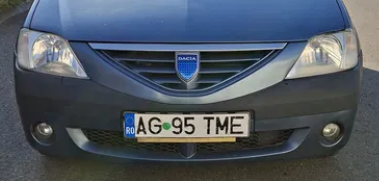
\includegraphics[width=\linewidth]{figures/AG95TME.png}
    \caption{Cadrul de intrare}
  \end{subfigure}
  \hfill
  \begin{subfigure}[c]{0.18\linewidth}
    \centering
    
\includegraphics[width=\linewidth]{figures/AG95TME.png_lp_0.jpg}
    \caption{Candidatul 1}
  \end{subfigure}
  \hfill
  \begin{subfigure}[c]{0.18\linewidth}
    \centering
    
\includegraphics[width=\linewidth]{figures/AG95TME.png_lp_1.jpg}
    \caption{Candidatul 2}
  \end{subfigure}
  \hfill
  \begin{subfigure}[c]{0.18\linewidth}
    \centering
    
\includegraphics[width=\linewidth]{figures/AG95TME.png_lp_2.jpg}
    \caption{Candidatul 3}
  \end{subfigure}
  \caption{Imaginea inițială și cele 3 elemente extrase în momentul rulării modulului de localizare cu \texttt{top\_k}$=3$.}
  \label{fig:rezultat_localizare}
\end{figure}

\subsubsection{Segmentarea caracterelor}
\indent\par
Etapa de segmentare primește candidații de plăcuță produși de etapa de localizare și are ca scop izolarea fiecărui caracter într-o imagine distinctă. Dintre tehnicile prezentate în capitolul~\ref{chap:segmentare}, a fost adoptată analiza contururilor, combinată cu utilizarea cunoștințelor apriori privind aspectul caracterelor. Această alegere a fost preferată unei abordări bazate pe analiza proiecțiilor care, deși oferă o reprezentare unidimensională compactă a distribuției pixelilor de prim-plan, depinde de existența unor văi suficient de adânci între caracterele adiacente. Pe plăcuțele reale, înclinarea de câteva grade și spațierea neuniformă a caracterelor fac ca aceste văi să se estompeze, fuzionând simboluri vecine într-un singur segment. Decizia la nivelul fiecărei componente conexe în parte rămâne, în schimb, independentă de unghiul de înclinare și de spațierea dintre simboluri, comportament confirmat de comparația cantitativă prezentată în secțiunea de experimente.

Pipeline-ul de segmentare începe cu restrângerea decupajului la corpul efectiv al plăcuței, eliminând contextul reținut eronat în etapa de localizare, precum fragmentele de caroserie sau cadrul plăcuței. Restrângerea se realizează fie prin selectarea celei mai mari componente conexe luminoase, corespunzătoare fundalului uniform al plăcuței, fie, atunci când aceasta nu este concludentă, prin detectarea benzii de caractere: elementele de înălțime plauzibilă sunt grupate după coordonata lor verticală, iar decupajul este redus la dreptunghiul de încadrare al grupului dominant.

Corpul astfel obținut este binarizat printr-un prag adaptiv gaussian în variantă inversată (\texttt{adaptiveThreshold}), care compensează variațiile locale de iluminare de-a lungul plăcuței, obținând caracterele drept prim-plan alb. Din imaginea binară se extrag contururile externe, iar dreptunghiurile lor de încadrare constituie casetele-candidat pentru caractere. Atunci când numărul de contururi este insuficient (sub trei), imaginea este erodată ușor, iar extragerea este reluată, separând caracterele unite accidental prin zgomot.

Casetele-candidat sunt apoi filtrate printr-o succesiune de criterii derivate din aspectul așteptat al unui caracter. Un prag de contrast intern, calculat ca abaterea standard a intensităților din interiorul casetei raportată la un prag Otsu determinat pe ansamblul casetelor, elimină regiunile uniforme precum reziduurile cadrului. Constrângerile de înălțime relativă (între $0{,}40$ și $0{,}95$ din înălțimea plăcuței) și de raport de aspect ($w/h$ între $0{,}08$ și $1{,}3$) elimină structurile prea mici sau cu geometrie implauzibilă, pragul inferior fiind suficient de permisiv pentru a păstra caractere înguste precum cifra \texttt{1}. În final, casetele care ating marginile laterale ale decupajului sunt respinse, anulând fragmentele de cadru tăiate, iar o trecere de consistență păstrează doar casetele a căror înălțime se află în jurul valorii mediane (între $0{,}55$ și $1{,}45$ din aceasta).

\begin{verbatim}
    thresholded = cv.adaptiveThreshold(
        greyscale, 255, cv.ADAPTIVE_THRESH_GAUSSIAN_C,
        cv.THRESH_BINARY_INV, block, 2)
    contours = self._helper.find_countours(
        thresholded, aspect_ratio_bounds=(0.04, 2.0))
    for c, s in zip(contours, stds):
        x, y, w, h = c
        if s < std_thr:
            continue
        if not (min_height <= h <= max_height):
            continue
        if not (min_w_h <= w / h <= max_w_h):
            continue
        if x < border_margin or (x + w) > (W - border_margin):
            continue
        kept.append((x, y, w, h))
\end{verbatim}

Caracterele lipite, care produc o singură casetă vizibil mai lată decât înaltă ($w > 1{,}2\,h$), sunt separate ulterior prin metoda \texttt{\_split\_wide\_blobs}: în interiorul casetei se calculează proiecția verticală pe coloane, iar tăierea se face în dreptul minimelor locale (văile dintre caractere), numărul de tăieturi fiind estimat din raportul de aspect al casetei. Spre deosebire de o abordare globală bazată pe proiecții, profilul este aici folosit strict local, pentru a împărți o regiune deja izolată, evitând astfel sensibilitatea profilului global la înclinarea plăcuței.

Deoarece etapa de localizare poate furniza mai mulți candidați de plăcuță, segmentarea este rulată pe fiecare dintre aceștia, iar setul de caractere reținut este cel care obține scorul maxim conform unei funcții de evaluare (\texttt{\_score}). Acest cuplaj prin parametrul \texttt{top\_k} transformă etapa de segmentare într-un mecanism de recuperare a erorilor de localizare: un candidat incorect (de exemplu o regiune de grilaj reținută eronat) va produce o segmentare cu un scor scăzut și va fi astfel respins în favoarea candidatului corect.

Funcția de evaluare valorifică o cunoștință apriori esențială: o plăcuță validă conține un număr cunoscut de caractere, de dimensiuni comparabile și dispuse pe aceeași linie de bază. Scorul integrează, în consecință, trei componente: abaterea numărului de casete detectate față de numărul așteptat (în jur de șapte simboluri pentru formatul autohton), consistența înălțimilor casetelor (caracterele unei plăcuțe au înălțimi similare) și alinierea lor verticală (caracterele împărtășesc aceeași linie de bază). O segmentare care satisface aceste constrângeri primește un scor ridicat, întrucât corespunde tiparului geometric al unei plăcuțe reale.

Rezultatul acestei etape este ilustrat în Figura~\ref{fig:rezultat_segmentare}: pornind de la plăcuța localizată în etapa anterioară, modulul izolează fiecare caracter într-o imagine distinctă, producând cele șapte simboluri care urmează a fi transmise individual etapei de recunoaștere.

\begin{figure}[H]
  \centering
  % TODO: înlocuiește numele fișierelor cu pozele finale
  \begin{subfigure}[b]{0.5\linewidth}
    \centering
    
\includegraphics[width=\linewidth]{figures/AG95TME.png_lp_0.jpg}
    \caption{Plăcuța localizată}
  \end{subfigure}

  \vspace{0.8em}

  \begin{subfigure}[b]{0.12\linewidth}
    \centering
    
\includegraphics[width=\linewidth]{figures/char_0.jpg}
  \end{subfigure}
  \hfill
  \begin{subfigure}[b]{0.12\linewidth}
    \centering
    
\includegraphics[width=\linewidth]{figures/char_1.jpg}
  \end{subfigure}
  \hfill
  \begin{subfigure}[b]{0.12\linewidth}
    \centering
    
\includegraphics[width=\linewidth]{figures/char_2.jpg}
  \end{subfigure}
  \hfill
  \begin{subfigure}[b]{0.12\linewidth}
    \centering
    
\includegraphics[width=\linewidth]{figures/char_3.jpg}
  \end{subfigure}
  \hfill
  \begin{subfigure}[b]{0.12\linewidth}
    \centering
    
\includegraphics[width=\linewidth]{figures/char_4.jpg}
  \end{subfigure}
  \hfill
  \begin{subfigure}[b]{0.12\linewidth}
    \centering
    
\includegraphics[width=\linewidth]{figures/char_5.jpg}
  \end{subfigure}
  \hfill
  \begin{subfigure}[b]{0.12\linewidth}
    \centering
    
\includegraphics[width=\linewidth]{figures/char_6.jpg}
  \end{subfigure}

  \caption{Rezultatul etapei de segmentare: plăcuța localizată (sus) și cele șapte caractere izolate (jos), fiecare extras într-o imagine distinctă.}
  \label{fig:rezultat_segmentare}
\end{figure}

\subsubsection{Recunoașterea caracterelor}
\indent\par
Ultima etapă a fluxului de procesare atribuie fiecărui caracter segmentat o etichetă, dintr-un alfabet de cifre și litere. Pentru această sarcină a fost ales un clasificator de tip SVM, ale cărui fundamente teoretice au fost prezentate în capitolul~\ref{chap:recunoastere}.

Fiecare caracter este adus la o reprezentare uniformă, independentă de dimensiunea sa originală. Imaginea este mai întâi adusă la o formă pătrată prin completarea laturii mai scurte cu o bordură, apoi redimensionată la o rezoluție fixă de $28 \times 28$ pixeli. Asupra acestei imagini se calculează un descriptor de tip HOG, pe o fereastră de $28 \times 28$ cu celule de $7 \times 7$ pixeli, blocuri de $14 \times 14$ cu pas de $7$ pixeli și $9$ intervale de orientare, rezultă un vector de $324$ de trăsături. Această reprezentare, care surprinde distribuția locală a orientărilor muchiilor în loc de intensitatea brută a pixelilor, constituie intrarea clasificatorului.

Predicția nu se reduce la atribuirea independentă a etichetei celei mai probabile fiecărui caracter, ci valorifică o cunoștință apriori privind formatul plăcuțelor. Atunci când numărul de caractere segmentate corespunde unui format cunoscut, decodarea se realizează poziție cu poziție, restrângând la fiecare poziție mulțimea etichetelor admise (cifră sau literă) și alegând eticheta cu marginea maximă raportată de funcția de decizie a clasificatorului. Pentru lungimile ambigue, în care același număr de caractere admite mai multe tipare, fiecare tipar este evaluat separat, iar varianta cu marginea medie cea mai mare este reținută. Suplimentar, atunci când segmentarea produce un caracter în plus față de un format așteptat, se încearcă și sub-secvențele obținute prin eliminarea pe rând a câte unui caracter, comparate tot pe baza marginii medii per poziție; astfel, un fragment supra-segmentat, care primește o margine apropiată de zero, este eliminat în favoarea tiparului care se potrivește curat. Dacă numărul de caractere nu corespunde niciunui format cunoscut, se revine la atribuirea neconstrânsă a etichetei celei mai probabile.

\subsection{Nivelul de aplicație}
\indent\par
Modulul de logică a aplicației constituie, alături de modulul de intrare, una dintre marginile extensibile ale sistemului. Rolul său este de a consuma rezultatul produs de fluxul de procesare și de a declanșa acțiunea corespunzătoare contextului de execuție.

\subsubsection{Sistem integrat}
\indent\par
În scenariul unui sistem integrat, modulul de logică a aplicației acționează direct asupra mediului fizic. O implementare reprezentativă este cea a unui punct de control al accesului, în care recunoașterea unui număr de înmatriculare aflat într-o listă de autorizare declanșează ridicarea unei bariere auto prin acționarea echipamentului \textit{hardware} corespunzător. Aceeași implementare poate emite, în paralel, notificări automate, de exemplu prin \textit{e-mail}, către un operator sau către un sistem de evidență, atât pentru accesele autorizate, cât și pentru tentativele neautorizate. Caracterul abstract al interfeței permite combinarea liberă a unor astfel de acțiuni, fără modificarea nucleului.

\subsubsection{Aplicație demo}
\indent\par
% DE SCHIMBAT
Pentru aplicația demonstrativă, modulul de logică a aplicației nu acționează asupra unui echipament fizic, ci expune rezultatele recunoașterii către un client extern. Implementarea se bazează pe biblioteca \textit{FastAPI}, care oferă infrastructura unui server web, și pe protocolul \textit{WebSocket}, ales pentru capacitatea sa de a menține o conexiune bidirecțională persistentă. Prin intermediul acestei conexiuni, rezultatele procesării sunt transmise în timp real către interfața clientului, pe măsură ce sunt produse de fluxul de procesare, fără a necesita interogări repetate din partea acestuia.

\chapter{Metrici și experimente}\label{chap:metrici}
\indent\par
Capitolul de față prezintă evaluarea experimentală a sistemului IORA, urmărind să cuantifice performanța fiecărei etape a fluxului de procesare, dar și a întregului lanț de recunoaștere. Mai întâi sunt descrise seturile de date utilizate, atât cel destinat evaluării \textit{end-to-end} a sistemului, cât și cel folosit pentru antrenarea clasificatorului de caractere, împreună cu procedeele de normalizare, adnotare și augmentare aplicate acestora. În continuare sunt introduse metricile de evaluare și sunt raportate rezultatele obținute, mai întâi pentru componenta de recunoaștere a caracterelor considerată izolat, apoi pentru sistem la nivel de etapă și \textit{end-to-end}. În final, secțiunea de experimente justifică, prin rezultate cantitative, principalele decizii de proiectare adoptate în fluxul de procesare și evidențiază contribuția fiecărei intervenții la performanța de ansamblu.

\section{Seturi de date}
\indent\par
Sistemul IORA operează cu două seturi de date distincte: un set de evaluare, utilizat pentru măsurarea performanței \textit{end-to-end} a fluxului de procesare, și un set de antrenare, destinat construirii clasificatorului SVM. Ambele gravitează în jurul aceluiași corpus de imagini cu plăcuțe de înmatriculare obținut prin platforma Roboflow~\cite{roboflow-lp-dataset}, completat, în cazul setului de evaluare, de o componentă românească colectată manual, iar în cazul setului de antrenare, de un set de date dedicat caracterelor individuale cu fonturi variate.

\subsection{Setul de evaluare}
\indent\par
Pentru a determina robustețea sistemului și capacitatea sa de adaptare la diverse formate ale numărului de înmatriculare a fost necesară crearea unui set de date mixt, în care sunt prezente atât autovehicule de pe teritoriul României, cât și vehicule din alte regiuni ale globului. Pentru prima componentă a setului de date în momentul de față nu există o sursă general valabilă și deschisă publicului larg, așadar imaginile reprezentative acestei părți au fost colectate manual de pe platforme de comerț auto online. Această procedură de salvare și utilizare a imaginilor este conformă cu reglementările GDPR, întrucât fotografiile au fost publicate în mod voluntar de către vânzători pe platforme cu acces liber, fiind astfel destinate publicului larg, iar prelucrarea lor s-a realizat strict în scop de cercetare și evaluare a sistemului. Pentru componenta internațională, a fost utilizat setul de date public obținut prin intermediul platformei Roboflow~\cite{roboflow-lp-dataset}.

\subsubsection{Normalizarea seturilor de date}
\indent\par
În contextul sistemelor de recunoaștere automată a numerelor de înmatriculare puse în funcțiune în cadrul parcărilor condițiile de execuție precum poziția numărului de înmatriculare, distanța și raportul dimensiunilor, unghiul de captare și distanța focală sunt bine cunoscute, permitând valorificarea lor în procesul de localizare.

Pentru a reproduce aceste condiții, a fost necesară normalizarea setului de date. În cazul imaginilor obținute în mod manual, acest procedeu a presupus selectarea autovehiculelor care prezentau un număr de înmatriculare vizibil, urmată de o decupare pentru a reduce zgomotul de fundal și a oferi o distanță focală relativ constantă. Un exemplu al procesului poate fi observat în figura~\ref{fig:normalizare_imagine_ro}, unde înainte de normalizare erau prezente elemente de zgomot agresive atât în parbrizul mașinii cât și în spațiul înconjurător.
\begin{figure}[H]
  \centering
  \begin{subfigure}[b]{0.45\textwidth}
    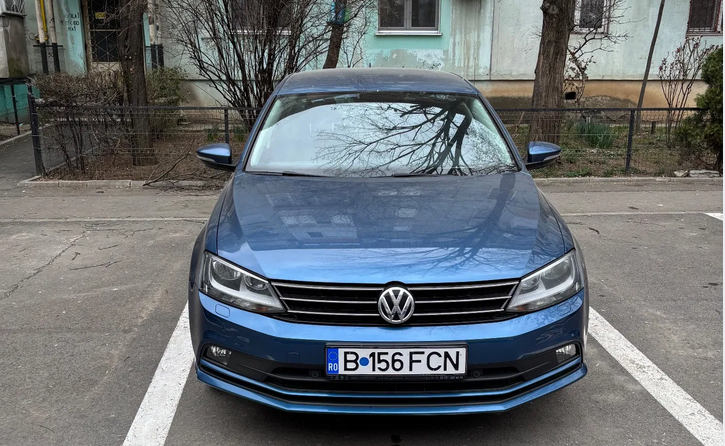
\includegraphics[width=\textwidth]{figures/b156fcn_initial.png}
    \caption{Înainte de normalizare}
    \label{fig:img_initiala}
  \end{subfigure}
  \hfill
  \begin{subfigure}[b]{0.45\textwidth}
    \includegraphics[width=\textwidth]{figures/b156fcn_cropped.png}
    \caption{După normalizare}
    \label{fig:img_decupata}
  \end{subfigure}
  \caption{Un exemplu de imagine alterată pentru a reduce zgomotul de fundal și normaliza unghiul de captură}
  \label{fig:normalizare_imagine_ro}
\end{figure}

Pentru componenta internațională a setului de date procesul a fost unul mai rapid, fiind necesară doar selectarea imaginilor corespunzătoare criteriilor menționate anterior. În figura~\ref{fig:normalizare_imagine_thl} se poate observa un exemplu de imagine corespunzătoare pusă în paralel cu o imagine care nu adera la standardele impuse.
\begin{figure}[H]
  \centering
  \begin{subfigure}[b]{0.45\textwidth}
    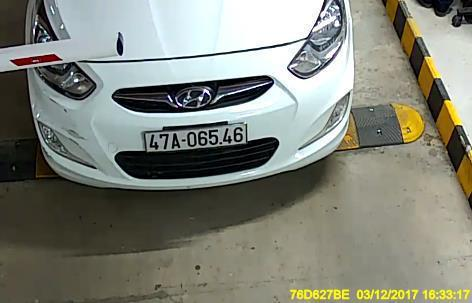
\includegraphics[width=\textwidth]{figures/imagine_buna_thl.jpg}
    \caption{Imagine corespunzătoare}
  \end{subfigure}
  \hfill
  \begin{subfigure}[b]{0.45\textwidth}
    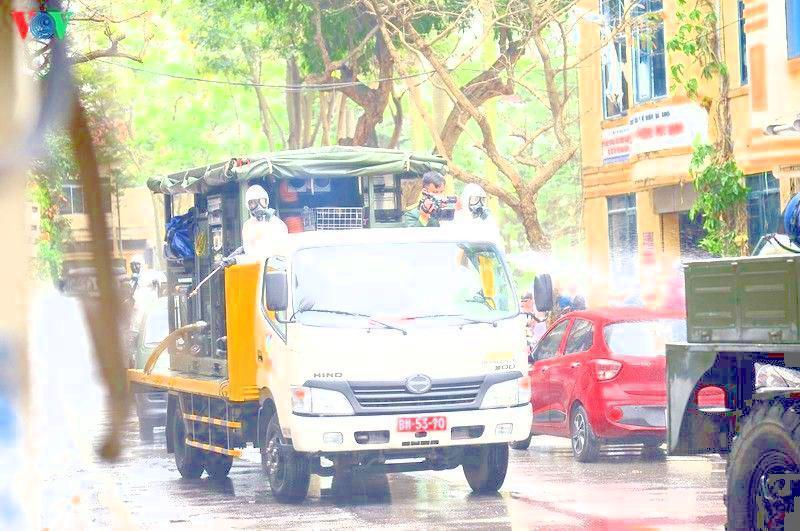
\includegraphics[width=\textwidth]{figures/imagine_proasta_thl.jpg}
    \caption{Imagine necorespunzătoare}
  \end{subfigure}
  \caption{Paralelă între o imagine conformă și una neconformă}
  \label{fig:normalizare_imagine_thl}
\end{figure}

\subsubsection{Crearea sursei de adevăr a setului de date}
\indent\par
Procedeul descris anterior constituie, însă, doar primul pas în construirea unui set de date potrivit strategiei de procesare propuse de această teză. Este în continuare necesară o sursă de adevăr uniformă pe componentele locală și internațională. Această secțiune prezintă pașii luați în completarea imaginilor cu informații relevante și conforme cu realitatea, care să reprezinte reperul față de care vor fi evaluate predicțiile generate de \textit{pipeline}.

Prima etapă este reprezentată de adnotarea imaginilor cu numărul de înmatriculare afișat în acestea, sarcină realizată manual, prin deschiderea lor rând pe rând, urmată de adăugarea valorilor într-un fișier \texttt{.csv} dedicat. Pentru a permite analizarea performanței componentei de localizare, a fost dezvoltat un utilitar \textit{software} dedicat extragerii chenarelor ce încadrează numerele de înmatriculare (\textit{bounding boxes}). Această aplicație cu interfață grafică facilitează delimitarea manuală a regiunii de interes, permițând utilizatorului să definească chenarul de încadrare prin marcarea coordonatelor aferente colțurilor din stânga-sus și dreapta-jos ale plăcuței.

\subsection{Setul de antrenare a clasificatorului SVM}
\indent\par
Antrenarea clasificatorului de caractere necesită un set de date format din imagini de caractere individuale, fiecare asociată cu eticheta sa. Construirea acestui set a urmat o strategie pe două surse: caractere generate automat prin aplicarea fluxului de procesare asupra imaginilor de antrenare din setul~\cite{roboflow-lp-dataset} de plăcuțe, urmate de etichetare manuală prin intermediul unei aplicații \textit{software} dedicate, și un set extern de caractere individuale extrase din imagini naturale, cu o mare diversitate de fonturi, scale și condiții de captură~\cite{deCampos09}. Combinarea celor două surse urmărește, pe de o parte, alinierea distribuției datelor de antrenare la caracteristicile particulare ale caracterelor segmentate de sistemul propriu și, pe de altă parte, asigurarea unui volum și a unei diversități tipografice suficiente.

\subsubsection{Generarea automată prin fluxul de procesare}
\indent\par
Prima sursă de data este generată prin intermediul sistemului cu ajutorul utilitarului~\textit{software} \texttt{generate\_dataset.py}

Acesta aplică asupra imaginilor de antrenare din componenta internațională a setului de plăcuțe etapele de localizare și segmentare descrise anterior, salvând caracterele segmentate drept imagini individuale, neetichetate. Integrarea acestui subset autogenerat în datele de antrenament a fost motivată de considerente practice: exemplele astfel obținute reflectă cu maximă fidelitate particularitățile și imperfecțiunile specifice extracției reale din sistem. Astfel, clasificatorul este expus la condiții realiste de operare, învățând să gestioneze variații ale unghiului de rotație, artefacte de segmentare sau caractere trunchiate.

\subsubsection{Sursă externă de caractere}
\indent\par
A doua sursă de date o constituie setul public \textit{Chars74K}~\cite{deCampos09}, introdus de de Campos și colaboratorii pentru problema recunoașterii caracterelor în imagini naturale. Dintre componentele acestui set a fost utilizat subsetul \texttt{EnglishImg}, care reunește $7705$ caractere segmentate din scene naturale, distribuite în $62$ de clase corespunzătoare cifrelor și literelor latine majuscule și minuscule (\texttt{0-9}, \texttt{A-Z}, \texttt{a-z}). Spre deosebire de caracterele produse de propriul \textit{pipeline}, aceste mostre provin din imagini reale, prezentând o variabilitate ridicată a fontului, a scalei și a condițiilor de iluminare, întrucât autorii au păstrat rezoluția originală a fiecărui caracter așa cum apare în imaginea-sursă.

Setul este distribuit deja etichetat și organizat ca un arbore de directoare, cu câte un director per clasă, fiecare caracter fiind salvat ca o imagine PNG individuală. Această structură permite integrarea directă a mostrelor în setul de antrenare, fără efort manual de adnotare. Rolul acestei surse este de a completa diversitatea tipografică a caracterelor autogenerate: în timp ce prima sursă aliniază distribuția datelor la particularitățile segmenterului propriu, Chars74K introduce o varietate mai amplă de forme și de fonturi întâlnite în condiții reale, contribuind la capacitatea de generalizare a clasificatorului.

\subsubsection{Etichetarea manuală}
\indent\par
Etichetarea mostrelor generate automat este realizată prin scriptul \texttt{label\_\-dataset.py}, care oferă o interfață minimală de etichetare asistată, construită cu ajutorul bibliotecii OpenCV. Fiecare imagine neetichetată este afișată succesiv, iar operatorul atribuie eticheta prin apăsarea tastei corespunzătoare caracterului. Apoi, imaginea este mutată automat în directorul clasei respective. Tasta dedicată permite marcarea mostrelor nevalide (caractere nerecunoscute sau segmentate eronat) prin mutarea lor într-un director special, în timp ce o altă tastă permite ignorarea unei mostre.

\subsubsection{Augmentarea setului prin rotații}
\indent\par
Deoarece setul de caractere etichetate manual prezenta un volum limitat și o variație redusă a înclinației, a fost necesară extinderea artificială a acestuia. Această etapă s-a realizat prin intermediul utilitarului software~\texttt{augment\_dataset}, care aplică fiecărui imagini o rotație în jurul centrului imaginii, la unghiurile de $\pm 3^\circ$ și $\pm 5^\circ$. Acest proces nu are doar scopul de a extinde mărimea setului de date, ci și de a forța clasificatorul să devină invariant la pertubații geometrice. Rezultatul procesului este vizibil în figura~\ref{fig:paralela_augmentare}.

\begin{figure}[H]
  \centering
  \begin{subfigure}[b]{0.45\textwidth}
    \centering
    
\includegraphics{figures/0020.png}
    \caption{Caracter înainte de aplicarea rotației}
  \end{subfigure}
  \hfill
  \begin{subfigure}[b]{0.45\textwidth}
    \centering
    
\includegraphics{figures/0020_aug_rot_n05.png}
    \caption{Caracter după aplicarea rotației}
  \end{subfigure}
  \caption{Paralelă între un caracter înainte și după transformare}
  \label{fig:paralela_augmentare}
\end{figure}

Variantele augmentate sunt salvate alături de originale, marcate printr-un sufix dedicat (\texttt{\_aug\_rot}), ceea ce permite distingerea ulterioară a mostrelor sintetice de cele reale. Prin multiplicarea cu factorul de cinci, setul de antrenare crește de la $1862$ la $9310$ mostre.

\subsubsection{Setul de date rezultat}
\indent\par
Prin consolidarea setului de caractere etichetate manual, cu sursa externă de date, a rezultat configurația finală a corpusului de antrenare. Frecvența de apariție a fiecărei clase în cadrul setului final este ilustrată în Figura~\ref{fig:distributia_caracterelor}.

\begin{figure}[H]
  \centering
  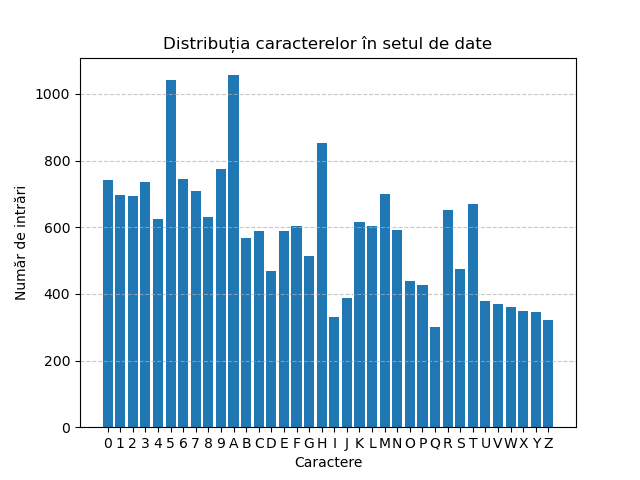
\includegraphics[width=\textwidth]{figures/set_date_plot.png}
  \caption{Distribuția caracterelor în setul de date final}
  \label{fig:distributia_caracterelor}
\end{figure}

\section{Testare și metrici}
\indent\par
Evaluarea sistemului urmărește două niveluri complementare: performanța componentei de recunoaștere a caracterelor, considerată izolat, și performanța întregului lanț de procesare, măsurată de la imaginea de intrare până la șirul de caractere recunoscut.


\subsection{Performanța componentei de recunoaștere a caracterelor}
\indent\par
Pentru evaluarea clasificatorului de caractere, setul de date este împărțit într-un subset de antrenare și unul de testare, în proporție de $80\%$, respectiv $20\%$. Împărțirea este stratificată, astfel încât distribuția claselor să fie păstrată în ambele subseturi.

Metricile raportate pentru clasificator sunt acuratețea globală și raportul de clasificare, care cuprinde, pentru fiecare clasă, precizia (\textit{precision}), rapelul (\textit{recall}) și scorul $F_1$. Aceste metrici sunt completate de matricea de confuzie, utilă pentru identificarea perechilor de caractere frecvent confundate (de exemplu cifra \texttt{0} și litera \texttt{O}, sau cifra \texttt{1} și litera \texttt{I}).

În urma antrenării clasificatorului statistic asupra setului de date menționat anterior au fost obținute următoarele rezultate generale pe subsetul de testare format din 4192 intrări:
\begin{itemize}
  \item \textbf{Acuratețe globală:} 96\%,
  \item \textbf{Precizie medie:} 96\%,
  \item \textbf{Rapel (\textit{Macro Recall}):} 95\%,
  \item \textbf{Scor mediu F1:} 96\%
\end{itemize}

Apropierea dintre valorile medii macro și acuratețea globală indică o performanță uniformă pe ansamblul claselor, fără simboluri defavorizate. Acest comportament este așteptat, întrucât setul combinat menține un volum suficient de exemplare pentru majoritatea claselor, evitând dezechilibrele. În ansamblu, o acuratețe de $96\%$ confirmă că reprezentarea liniarizată a imaginii, combinată cu nucleul RBF (\textit{Radial Basis Function} - Funcție de bază radială), captează suficientă informație distinctivă pentru separarea celor $36$ de clase.

Structura matricei de confuzie poate fi observată în figura~\ref{fig:matrice_confuzie}. Erorile sunt rare și concentrate într-un număr restrâns de perechi de simboluri. Deși rare, erorile persistă în urma procesului de antrenare, în mod special la perechile de caractere care prezintă o similitudine a formei geometrice: pentru perechea formată din cifra \texttt{0} și litera \texttt{O} există 14 erori care apar în mod simetric. De asemenea, există confuzii pentru următoarele perechi: litera \texttt{G} și \texttt{C}, cifra \texttt{1} și litera \texttt{I} sau \texttt{T}.

Aceste confuzii nu au, însă, o pondere uniformă în contextul aplicației. Confuziile de tip cifră-literă, precum \texttt{0}-\texttt{O} sau \texttt{1}-\texttt{I}, sunt în principiu recuperabile: poziția unui simbol în cadrul numărului de înmatriculare determină, conform formatului, dacă acesta trebuie să fie o cifră sau o literă, astfel încât o etapă ulterioară de decodare de format poate valorifica această cunoștință apriori pentru a le clarifica. În schimb, confuziile de tip literă-literă (\texttt{G}-\texttt{C}, \texttt{I}--\texttt{T}) rămân nerezolvabile și constituie limita erorilor clasificatorului.

\begin{figure}[H]
  \centering
  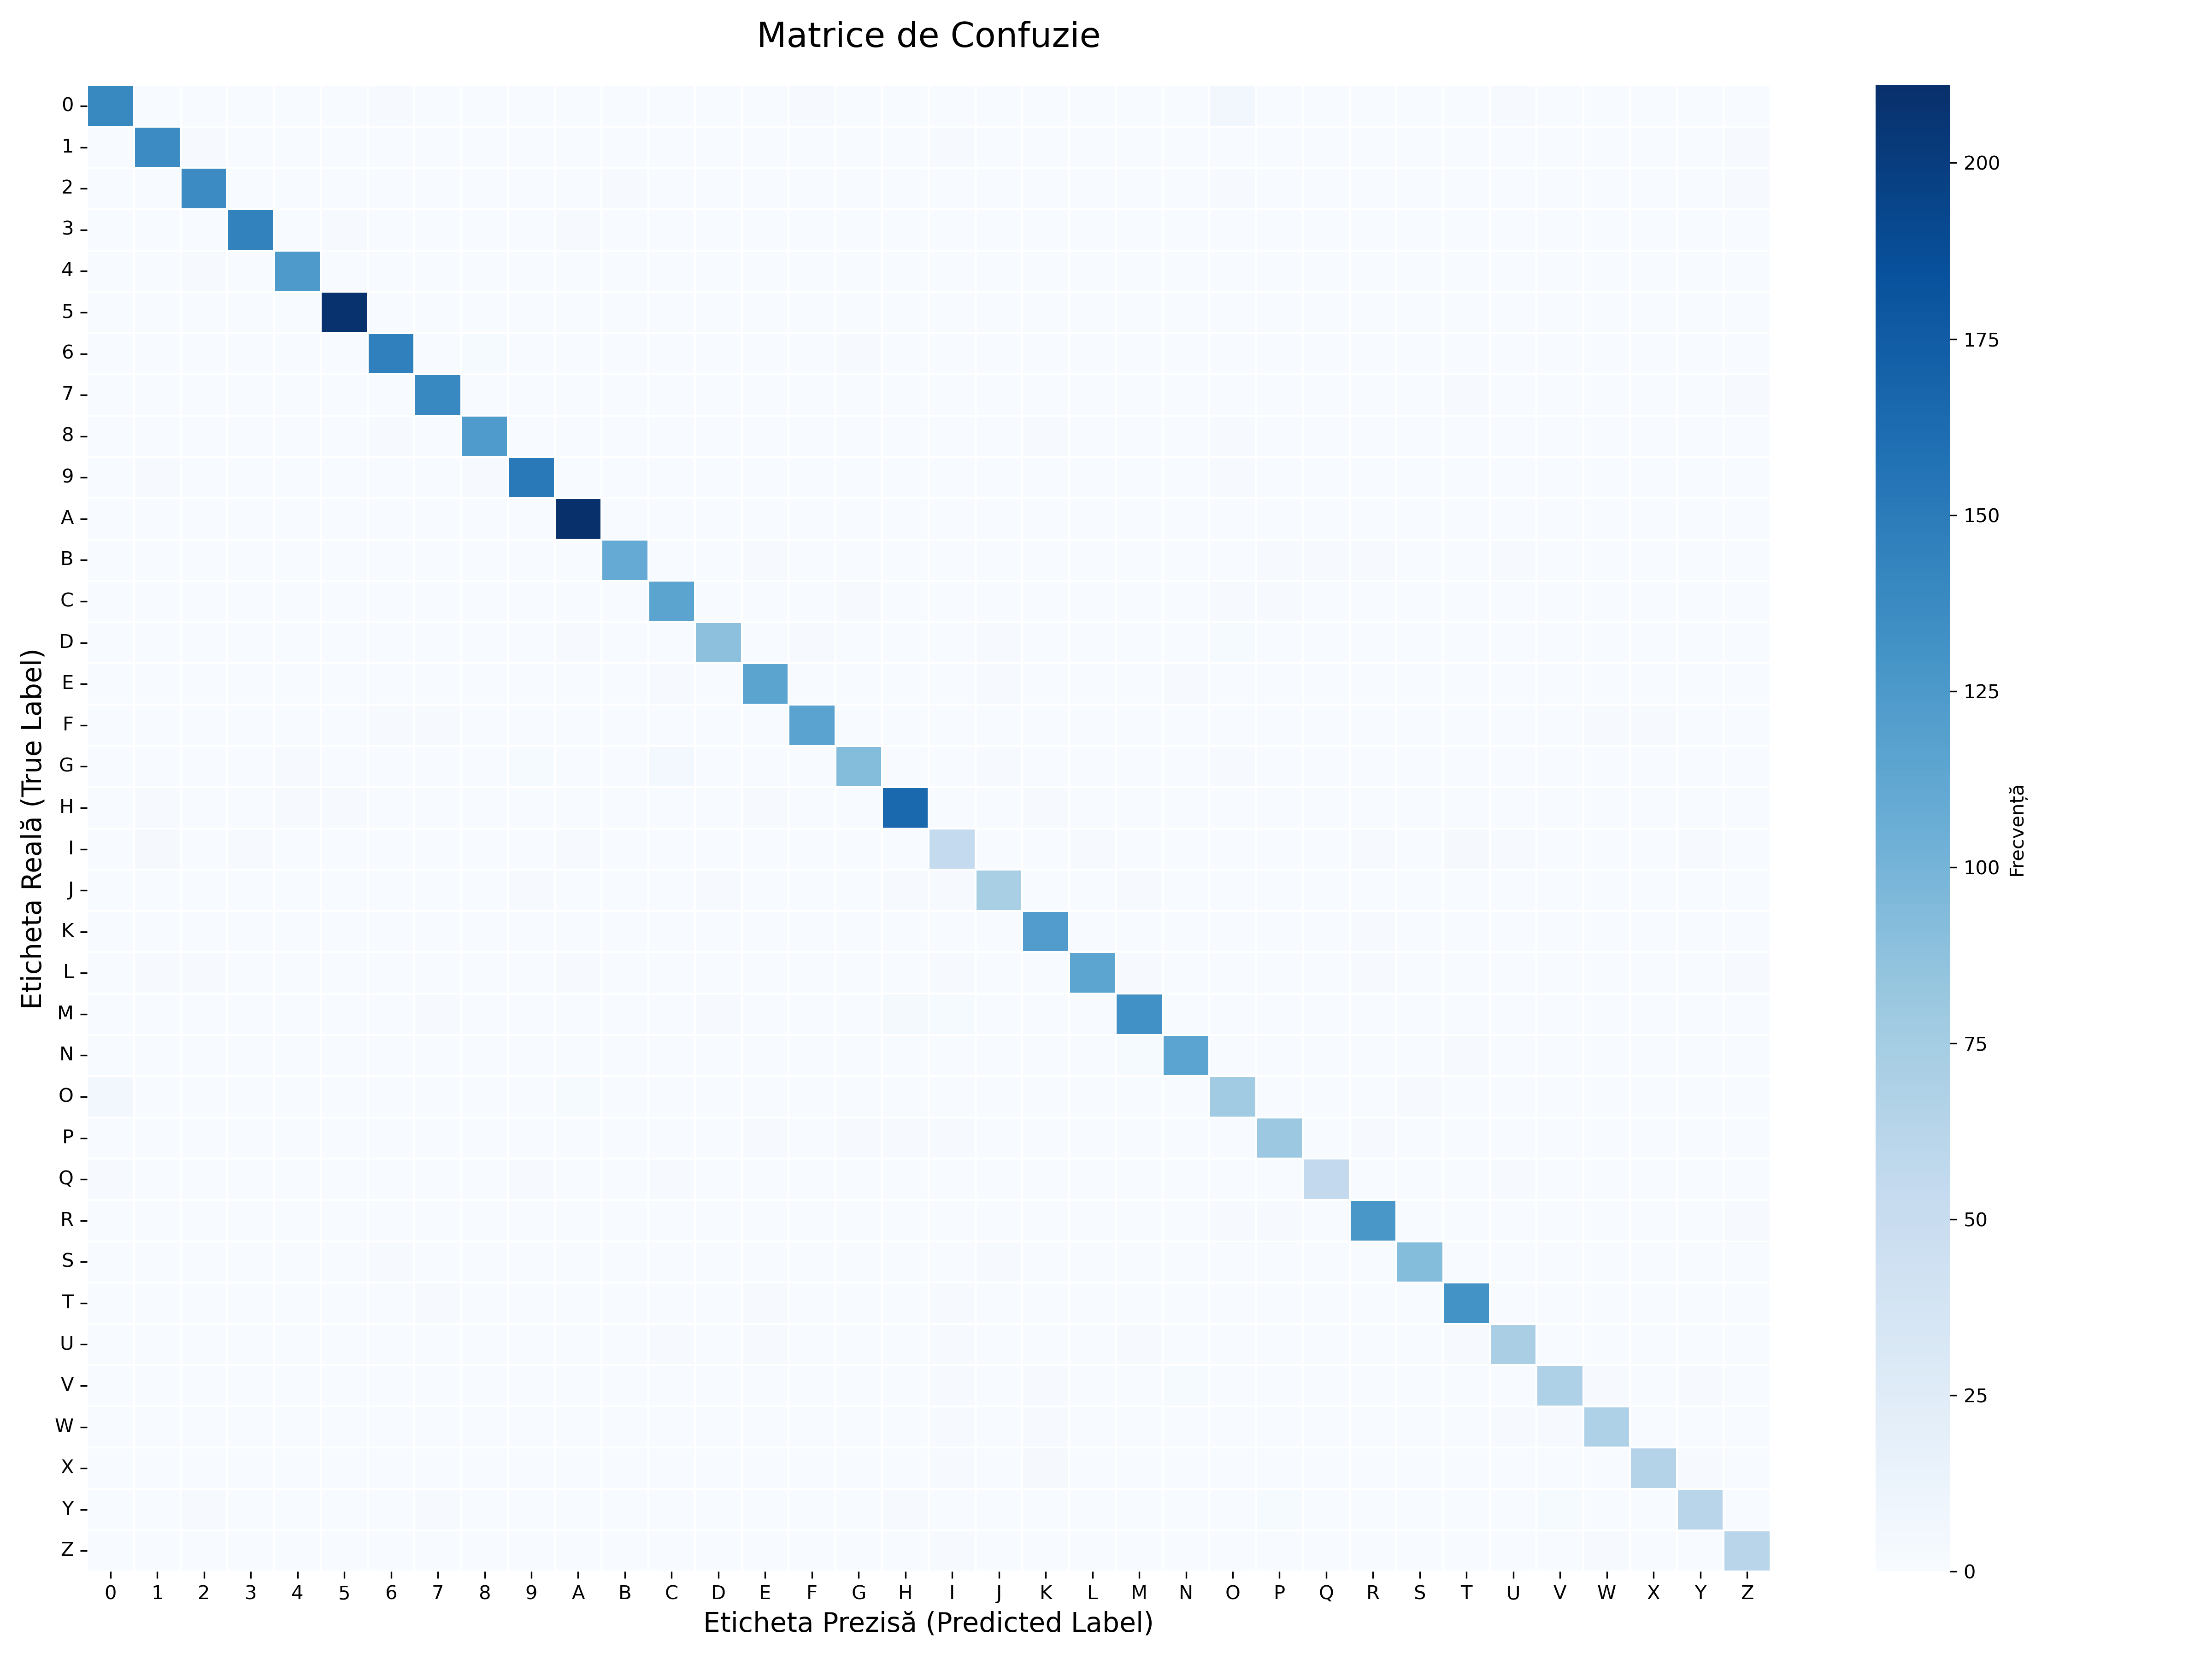
\includegraphics[width=\textwidth]{figures/matrice_confuzie.png}
  \caption{Matricea de confuzie obținută în urma antrenării clasificatorului}
  \label{fig:matrice_confuzie}
\end{figure}

\subsection{Performanța întregului sistem}
\indent\par
Pe lângă evaluarea izolată a clasificatorului, sistemul este evaluat și la nivel de etapă: rata de localizare corectă a plăcuței, rata de segmentare corectă a caracterelor și, în final, metrica integrată (\textit{end-to-end}), reprezentată de proporția plăcuțelor citite corect în întregime. Această din urmă metrică reflectă cel mai fidel performanța percepută a sistemului, întrucât o singură eroare la nivel de caracter invalidează întregul rezultat.

Înainte de a continua cu detaliile tehnice și numerice ale metricilor, este necesară clarificarea metodologiei de evaluare. După cum am menționat în cadrul secțiunii dedicate seturilor de date, colecția destinată evaluării sistemului cuprinde două componente: una internațională, formată din numere de înmatriculare din Thailanda, și una locală, cu numere din România. Astfel, pentru a obține rezultate fidele asupra performanței, utilitarul software \path{src/tools/evaluate.py} a fost rulat în mod separat asupra celor două componente.

Rularea separată a fost necesară și pentru că modulul de recunoaștere a caracterelor a fost adaptat să valorifice o cunoștință apriori esențială: structura formatului numărului de înmatriculare. Întrucât poziția fiecărui simbol determină, conform formatului regional, dacă acesta trebuie să fie cifră sau literă, metoda \texttt{predict} a clasei \texttt{CharacterRecognition} înlocuiește predicția top-1 a SVM-ului cu marginile furnizate de \texttt{decision\_function} și restrânge subsetul de clase admis de format. Această decodare condiționată recuperează tocmai confuziile de tip cifră-literă discutate anterior (\texttt{0}-\texttt{O}, \texttt{1}-\texttt{I}), care altfel ar invalida întregul șir.

\subsubsection{Evaluarea localizării corectă a plăcuței}
\indent\par
Pentru a putea cuantifica proporția în care sistemul extrage în mod corect regiunea de interes ce conține numărul de înmatriculare, a fost folosită metrica \textit{Intersecție supra Reuniune} (IoU - \textit{Intersection over Union}). Pentru a calcula această metrică, este nevoie atât de regiunile delimitate de sistem drept zone candidate, cât și de coordonatele reale ale plăcuței (regiunea adnotată manual).

Deoarece modulul de localizare propune mai multe regiuni candidat pentru o singură imagine, evaluarea performanței se face doar raportat la zona cu cel mai mare raport IOU. Astfel, o imagine pentru care există cinci predicții posibile pentru regiunea de interes, va fi redusă la un singur rezultat IOU. Această abordare a fost aleasă deoarece, precum am menționat în capitolul anterior, modulul de segmentare extrage implicit zona ideală, mai exact zona cu cel mai mare IOU.

În urma rulării celor două utilitare software, \path{src/tools/evaluate.py} și \path{src/tools/metrics.py}, modulul de localizare obține un IoU mediu de $\approx0.65$ pe componenta internațională și $\approx0.63$ pe cea locală. Valorile moderate se explică prin natura modulului de extracție: etapele de dilatare orizontală și de fuziune a candidaților extind în mod deliberat regiunea propusă, pentru a garanta că plăcuța nu este fragmentată și că toate caracterele rămân în interiorul zonei de interes. Deoarece metrica IoU penalizează în egală măsură surplusul și deficitul de suprafață, o margine de câțiva pixeli în jurul plăcuței reduce sensibil scorul, chiar și atunci când localizarea este corectă din punct de vedere funcțional. Această explicație este confirmată practic de creșterea scorului IoU la $\approx0.80$ în momentul introducerii unei etape de validare cu un prag minim de încredere de $0.50$.

\subsubsection{Evaluarea segmentării caracterelor}
\indent\par
Spre deosebire de localizare, pentru care există o adnotare manuală a regiunii de interes, etapa de segmentare nu dispune de o delimitare de referință a fiecărui caracter în parte. Din acest motiv, evaluarea segmentării se realizează indirect, prin compararea numărului de caractere extrase de sistem cu lungimea șirului de referință al plăcuței. Metrica adoptată este acordul la nivel de număr de caractere: pentru fiecare imagine, raportul dintre minimul și maximul celor două valori, după cum este prezentat în Ecuația \ref{eq:acord_caractere}.

\begin{equation}
    \text{Acord} = \frac{\min(n_{\text{seg}}, n_{\text{gt}})}{\max(n_{\text{seg}}, n_{\text{gt}})}
    \label{eq:acord_caractere}
\end{equation}

\noindent unde $n_{\text{seg}}$ este numărul de caractere segmentate, iar $n_{\text{gt}}$ este numărul de simboluri din adevărul de referință. Valoarea $1$ indică un acord perfect, iar abaterile, fie prin sub-segmentare, fie prin supra-segmentare reduc proporțional scorul. Această metrică surprinde corectitudinea structurală a segmentării fără a presupune o adnotare la nivel de caracter.

Pentru componenta internațională, etapa de segmentare a obținut un acord mediu de $\approx0.85$, iar pentru cea locală de $\approx0.82$. Interpretarea acestor valori sugerează că, în mare parte, modulul de segmentare extrage un număr apropiat de caractere relativ la sursa de adevăr. Diferența rămasă până la acordul perfect este atribuibilă, pe de o parte, plăcuțelor pentru care etapa de localizare a furnizat un decupaj imperfect, iar pe de altă parte cazurilor de fuziune a caracterelor adiacente sau de fragmentare a caracterelor cu structură discontinuă.

\subsubsection{Evaluare E2E}
\indent\par
Metrica integrată (\textit{end-to-end}) reflectă cel mai fidel performanța percepută a sistemului, întrucât consideră corectă o plăcuță doar atunci când întregul șir de caractere coincide cu adevărul de referință. O singură eroare la nivel de caracter, indiferent de poziția sa, invalidează rezultatul. Pentru a completa această măsură binară, evaluarea raportează și \emph{similaritatea Levenshtein} a șirului recunoscut față de cel de referință, o metrică mai fină care surprinde gradul de corectitudine parțială a predicțiilor invalidate.

Evaluarea pe componenta internațională a setului de date a indicat o acuratețe de $\approx0{,}69$, în timp ce pentru componenta națională s-a obținut un procentaj de $\approx0{,}73$. Similaritatea Levenshtein medie depășește în ambele cazuri pragul de $\approx0{,}80$. Această valoare, semnificativ mai ridicată decât rata de potrivire exactă, confirmă faptul că o proporție importantă a predicțiilor invalidate diferă de adevărul de referință printr-un singur caracter. Cel mai adesea, aceste erori punctuale sunt cauzate de posibilele confuzii vizuale ale modulului de recunoaștere, sau diferitele artefacte vizuale prezente pe o plăcuță, evidențiate în Figura~\ref{fig:artefacte}

\begin{figure}[H]
  \centering
  \begin{subfigure}[b]{0.48\textwidth}
    \centering
    
\includegraphics[width=\textwidth]{figures/B934ATN.png_lp_1.jpg}
    \caption{Bulină albastră care va fi segmentată în mod incorect drept un caracter}
  \end{subfigure}
  \hfill
  \begin{subfigure}[b]{0.48\textwidth}
    \centering
    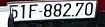
\includegraphics[width=\textwidth]{figures/CarLongPlate60_jpg.rf.9ac70cfc36770f5233142a727c52d534.jpg_lp_0.jpg}
    \caption{Artefact care blochează parțial numărul de înmatriculare}
  \end{subfigure}
  \caption{Exemple de artefacte ce pot deteriora procesul de recunoaștere}
  \label{fig:artefacte}
\end{figure}

\section{Experimente}
\indent\par
Experimentele prezentate în această secțiune urmăresc să justifice, prin rezultate cantitative, deciziile de proiectare adoptate în fluxul de procesare și să evidențieze contribuția fiecărei componente la performanța de ansamblu. Ele sunt organizate în trei părți: comparația dintre două abordări ale etapei de localizare, comparația dintre cele două abordări ale etapei de segmentare și seria de îmbunătățiri progresive aduse fluxului de recunoaștere.

\subsection{Comparația abordărilor de localizare}
\indent\par
Înainte de adoptarea abordării bazate pe operatorul Sobel și pe operațiile morfologice descrise anterior, etapa de localizare a fost implementată într-o manieră similară, dar cu un discriminant principal al regiunilor complet diferit: varianta inițială se baza pe aproximarea poligonală a contururilor.

Lanțul de preprocesare urma aceiași pași ca varianta curentă: conversia în tonuri de gri a cadrului primit de la modulul de intrare, atenuarea zgomotului și binarizarea, cu două deosebiri: reducerea zgomotului se realiza printr-un operator diferit de filtrul median, iar accentuarea muchiilor folosea detectorul de contururi Canny în locul operatorului Sobel. Extragerea contururilor (\texttt{findContours}) era identică cu cea din varianta curentă, însă selecția primilor \texttt{top\_k} candidați se făcea pe baza aproximării poligonale (\texttt{approxPolyDP}). Acest discriminant s-a dovedit însă nefiabil: în practică, multe dintre plăcuțe erau extrase ca poligoane cu un număr ridicat de laturi, ratând astfel criteriul geometric al formei dreptunghiulare. Tabelul~\ref{tab:cmp-localizare} sintetizează diferența de performanță dintre cele două abordări.

\begin{table}[H]
  \centering
  \begin{tabular}{lc}
    \hline
    Metodă de localizare & IoU mediu \\
    \hline
    Aproximare poligonală (\texttt{approxPolyDP}, variantă explorată) & $< 0{,}40$ \\
    Sobel + morfologie + \texttt{top\_k} (abordarea propusă) & $\approx0{,}60$ \\
    \hline
  \end{tabular}
  \caption{Comparație între cele două abordări ale etapei de localizare, evaluate prin același lanț de selecție \texttt{top\_k} și corecție de înclinare.}
  \label{tab:cmp-localizare}
\end{table}

Abordarea bazată pe aproximare poligonală nu a reușit să depășească un IoU mediu de $0{,}40$, în timp ce abordarea curentă atinge aproximativ $0{,}60$. Cauza principală a limitării este dependența de detectarea unui contur închis și dreptunghiular al marginii plăcuței: în condiții reale, această margine este frecvent fragmentată, astfel încât aproximarea poligonală fie nu produce un patrulater, fie îl produce deplasat față de plăcuța reală. Spre deosebire de aceasta, abordarea bazată pe Sobel și operații morfologice nu depinde de conturul marginii plăcuței, ci de concentrarea de muchii verticale generate de caractere: un semnal mai robust și independent de calitatea conturului exterior.

\subsection{Comparația abordărilor de segmentare}
\indent\par
Pentru etapa de segmentare au fost considerate două dintre abordările prezentate în capitolul~\ref{chap:segmentare}: segmentarea bazată pe proiecții orizontale și verticale și cea bazată pe contururi, ghidată de cunoștințe apriori privind aspectul caracterelor. Înainte de detalierea tehnică a celor două, tabelul~\ref{tab:cmp-segmentare} sintetizează diferența de performanță dintre ele, diferență care a fundamentat alegerea abordării pe contururi.

\indent\par
\begin{table}[H]
  \centering
  \begin{tabular}{lccc}
    \hline
    Metodă de segmentare & Localizare & Segmentare & End-to-end \\
    \hline
    Bazată pe proiecții (variantă explorată) & 0{,}65 & 0{,}20 & 0{,}05 \\
    Bazată pe contururi (implementarea propusă) & 0{,}65 & 0{,}85 & 0{,}69 \\
    \hline
  \end{tabular}
  \caption{Comparație directă între cele două abordări ale etapei de segmentare, pe același set de candidați produși de etapa de localizare.}
  \label{tab:cmp-segmentare}
\end{table}

Aceste diferențe uriașe nu provin dintr-un avantaj al setului care să favoritizeze metodele bazate pe contururi, ci din modul în care fiecare abordare tratează semnalul.

Analiza proiecțiilor comprimă imaginea binară într-un profil unidimensional, obținut prin însumarea pixelilor de prim-plan pe coloane, iar separarea caracterelor depinde de existența unor văi suficient de adânci între vârfurile asociate fiecărui simbol. Pe plăcuțele din setul de evaluare, această condiție este rar îndeplinită: reziduurile cadrului (banda UE, șuruburile de prindere) și, mai ales, înclinarea de câteva grade a plăcuței determină suprapunerea pe verticală a coloanelor caracterelor adiacente, astfel încât văile dintre ele nu mai coboară sub pragul de extragere a vârfurilor.

Abordarea bazată pe contururi nu este afectată de acest fenomen, întrucât decide la nivelul fiecărei componente conexe în parte, izolând fiecare caracter prin propriul contur închis, independent de unghiul de înclinare și de spațierea dintre simboluri.

\subsection{Îmbunătățiri progresive ale fluxului de recunoaștere}\label{sec:imbunatatiri}
\indent\par
Plecând de la configurația de bază descrisă în secțiunile anterioare, au fost adoptate, succesiv, cinci intervenții incrementale care vizează etapele de segmentare, decodare și clasificare. Evaluarea s-a făcut pe setul de date dedicat evaluării sistemului, iar metricile raportate sunt rata \textit{end-to-end} (egalitate exactă), similaritatea Levenshtein a OCR-ului, acordul la nivel de număr de caractere segmentate și IoU-ul localizării. Tabelul~\ref{tab:imbunatatiri} sintetizează contribuția cumulativă a fiecărei intervenții.

\begin{table}[H]
  \centering
  \small
  \begin{tabular}{p{6.2cm}cccc}
    \hline
    Configurație & End-to-end & OCR sim. & Acord seg. & IoU \\
    \hline
    Bază & 0{,}489 & 0{,}768 & 0{,}809 & 0{,}588 \\
    \quad + reconstrucția segmentării  & 0{,}597 & 0{,}801 & 0{,}839 & 0{,}588 \\
    \quad + decodare condiționată de format & 0{,}645 & 0{,}801 & 0{,}839 & 0{,}588 \\
    \quad + trăsături HOG pentru SVM & 0{,}667 & 0{,}807 & 0{,}839 & 0{,}588 \\
    \quad + pre-procesare cu conservarea proporțiilor & 0{,}677 & 0{,}806 & 0{,}839 & 0{,}588 \\
    \quad + padding LP și augmentare cu rotații & \textbf{0{,}694} & 0{,}813 & 0{,}843 & 0{,}589 \\
    \hline
  \end{tabular}
  \caption{Contribuția cumulativă a celor cinci intervenții. Fiecare linie include modificările liniilor anterioare. Cumulat, rata end-to-end a crescut cu $20{,}5$ puncte procentuale ($91 \to 129$ plăcuțe corecte din $186$).}
  \label{tab:imbunatatiri}
\end{table}

\subsubsection{Reconstrucția etapei de segmentare}
\indent\par
Înainte de intervenție, decupajul de plăcuță era binarizat direct, iar contururile externe erau filtrate exclusiv prin raportul de aspect $w/h$, cu un prag inferior de $0{,}15$. Matricea de confuzii a arătat două surse sistematice de erori: aproximativ $250$ de caractere lipsă (dominate de $5\to\emptyset$ cu $55$ de cazuri, $1\to\emptyset$ cu $48$ de cazuri) și aproximativ $30$ de caractere inserate fals ($\emptyset\to A$, $\emptyset\to T$, $\emptyset\to H$). Caracterul \texttt{1}, cu un raport real $w/h$ între $0{,}07$ și $0{,}12$, era respins în întregime de pragul geometric, iar reziduurile cadrului plăcuței (banda UE, șuruburile de prindere) produceau contururi care imitau caractere reale.

Soluția a constat în (1) restrângerea decupajului la cea mai mare componentă conexă deschisă din interiorul plăcuței, eliminând cadrul înainte de binarizare; (2) coborârea pragului $w/h$ la $0{,}08$, recuperând caracterul \texttt{1}; (3) respingerea contururilor care ating marginile laterale ale plăcuței tăiate, anulând patternul de inserții; (4) o trecere de consistență pe înălțimi, care elimină casetele aflate în afara intervalului $[0{,}55\,m, 1{,}45\,m]$, unde $m$ este înălțimea mediană a supraviețuitorilor; (5) un divizor de blocuri largi care, pentru casete cu $w > 1{,}2\,h$, taie la coloana cu cea mai joasă proiecție verticală, recuperând caracterele lipite. Inserțiile au scăzut de la $\sim 30$ la $\sim 5$, iar rata end-to-end a urcat cu $10{,}8$ puncte procentuale.

Au fost respinse explicit aplicarea unei închideri morfologice $3\times3$, care, pe plăcuțe de $\sim 27$ de pixeli înălțime, a unit caracterele adiacente (numărul de contururi crude a scăzut de la $23$ la $4$ într-un caz observat), și varianta verticală $(2,1)$, cu același efect în formă atenuată.

\subsubsection{Decodare condiționată de format}
\indent\par
Analiza matricii de confuzie a indicat substituții frecvente între clase vizual similare (\texttt{4}$\to$\texttt{F}, \texttt{O}$\to$\texttt{0}, \texttt{1}$\to$\texttt{I}), generate de ambiguitatea internă a SVM-ului. Indiferent de regiune, structura numărului de înmatriculare oferă tocmai acest context: formatul fixează, pentru fiecare poziție, dacă simbolul așteptat este o cifră sau o literă. Cunoștințele pre-existente asupra formatului pot facilita procesul de clasificare, restrângând domeniul de predicții posibile.

Modificarea, localizată în metoda \texttt{predict} a clasei \texttt{CharacterRecognition}, este formulată independent de un format anume. Ea înlocuiește predicția top-1 a SVM-ului cu marginile furnizate de \texttt{decision\_function} și restrânge și restrânge subsetul de clase admis de format.

Atunci când o lungime dată admite mai multe formate candidate, fiecare șablon este evaluat, iar cel cu marginea medie pe poziție cea mai mare este selectat. Pentru lungimile care nu corespund niciunui format, decodarea revine la varianta neconstrânsă, evitând orice regresie. Aceeași logică se aplică nemodificat atât plăcuțelor românești și thailandeze.

\subsubsection{Trăsături HOG pentru clasificator}
\indent\par
Reprezentarea pe $784$ de dimensiuni (intensitățile brute ale pixelilor $28\times28$) a fost înlocuită cu un descriptor HOG.

Modelul a fost re-antrenat, atingând o acuratețe de $97\%$ pe subsetul independent. În pipeline-ul integrat, rata \textit{end-to-end} a urcat cu $2{,}2$ puncte procentuale (la $66{,}7\%$). Un alt rezultat este scăderea numărului de perechi de erori din matricea de confuzie de la $82$ la $70$, indicând o concentrare a acestora în categorii mai bine definite și mai ușor de abordat în continuare.

\subsubsection{Păstrarea proporțiilor caracterului}
\indent\par
Ultima modificare rezolvă o limitare a etapei de pregătire a caracterului: redimensionarea directă la $28\times28$ deforma raportul de aspect al claselor înguste. Un caracter \texttt{1}, cu $w/h \approx0{,}12$ la segmentare, devenea un pătrat, iar descriptorul HOG raporta o distribuție de orientări similară cu cea a unui \texttt{I}, \texttt{T} sau \texttt{L}. Modificarea din logica funcției \texttt{preprocess\_char} completează imaginea cu o margine constantă până la un pătrat, înainte de redimensionarea la $28\times28$.


\subsubsection{Augmentare cu rotații a setului de antrenare}
\indent\par
Schimbarea descrisă în cele ce urmează are drept scop creșterea robusteții clasificatorului la diferența dintre distribuția setului de antrenare și cea din mediul de execuție. Această ajustare a urcat rata end-to-end cu $1{,}7$ puncte procentuale (la $69{,}4\%$).

Intervenția constă într-un script de augmentare (\texttt{src/augment\_dataset.py}) care, pentru fiecare exemplar etichetat din setul obținut în mod manual, generează patru variante rotite la $\pm 3^\circ$ și $\pm 5^\circ$ în jurul centrului, cu marginea completată prin aceeași metodă \texttt{preprocess\_char}). Setul de antrenament crește astfel de la $1862$ la $9310$ mostre.

\subsubsection{Bilanț}
\indent\par
Cumulat, cele cinci intervenții au urcat rata \textit{end-to-end} de la $48{,}9\%$ la $69{,}4\%$. Două limitări reziduale rămân vizibile: tăierea caracterului inițial al plăcuței, cauzată în etapa de localizare și un set restrâns de substituții vizual ambigue dintre litere sau dintre cifre (\texttt{Y}$\to$\texttt{M}, \texttt{F}$\to$\texttt{6}, \texttt{1}$\to$\texttt{I}).

\chapter{Concluzii și perspective de viitor}
\label{chap:concluzii}

\paragraph{}
Acest capitol final recapitulează contribuțiile lucrării și rezultatele obținute, după care discută limitările sistemului și direcțiile în care acesta poate fi extins.

\section{Concluzii}

\paragraph{}
Obiectivul lucrării a fost construirea unui sistem de recunoaștere automată a numerelor de înmatriculare care să funcționeze fiabil pe o varietate largă de formate și să respecte o constrângere de timp real, folosind exclusiv tehnici clasice de viziune artificială și un clasificator SVM, fără a recurge la rețele neuronale profunde. Sistemul IORA, structurat pe trei etape: localizare, segmentare și recunoaștere, arată că o astfel de abordare rămâne viabilă atunci când este completată cu cunoștințe apriori despre structura problemei.

Un prim aspect confirmat de experimente este superioritatea criteriilor geometrice față de cele dependente de aparență. Renunțarea la segmentarea pe culoare a permis generalizarea la cele patru combinații cromatice admise în România și la formatele internaționale, întrucât raportul de aspect al regiunii este un descriptor mult mai stabil decât o paletă cromatică fixă. Aceeași concluzie se confirmă la nivelul segmentării: decizia luată independent pe fiecare componentă conexă rămâne robustă la înclinarea plăcuței, în timp ce analiza proiecțiilor cedează în prezența văilor estompate dintre caractere (un acord de $0{,}85$ față de $0{,}20$).

Al doilea aspect ține de rolul decisiv al cunoștințelor apriori. În absența unui model profund, performanța depinde de modul în care este exploatată structura numărului de înmatriculare. Decodarea condiționată de format, care restrânge la fiecare poziție mulțimea etichetelor admise, recuperează confuziile de tip cifră-literă (\texttt{0}-\texttt{O}, \texttt{1}-\texttt{I}) care altfel ar invalida întregul șir. Tot pe cunoștințe apriori se sprijină și cuplajul dintre localizare și segmentare: returnarea mai multor candidați de plăcuță transformă etapa de segmentare într-un mecanism de recuperare a erorilor de localizare, fără un cost de calcul suplimentar semnificativ.

Cantitativ, clasificatorul SVM antrenat pe descriptori HOG cu nucleu RBF a atins o acuratețe de $96\%$ pe cele $36$ de clase de caractere, iar seria de intervenții incrementale aplicate fluxului a urcat rata \textit{end-to-end} de la $48{,}9\%$ la $69{,}4\%$. Similaritatea Levenshtein medie depășește $0{,}80$, ceea ce arată că majoritatea erorilor rămase se reduc la un singur caracter greșit. Dincolo de metrici, sistemul este integrat într-o aplicație funcțională, organizată pe trei module decuplate prin interfețe și structuri de date proprii, care poate fi rulată atât pe un sistem integrat, cât și ca serviciu web, fără modificarea nucleului de procesare.

Merită subliniat că aceste rezultate au fost obținute pe un set de evaluare eterogen. Deși componentele locală și internațională au fost curățate și normalizate manual, ele rămân departe de a fi uniforme: persistă diferențe importante de unghi de captură, distanță, iluminare, font și calitate a imaginii. Într-un scenariu de exploatare precum cel vizat, un punct de control al accesului auto într-o parcare, aceste variabile sunt, în schimb, fixe și cunoscute: poziția camerei, distanța focală, unghiul și dimensiunea relativă a plăcuței nu variază de la un cadru la altul. Într-un asemenea cadru controlat, în care sistemul poate fi calibrat o singură dată pentru condițiile concrete de instalare, performanța reală ar fi sensibil mai ridicată decât cea măsurată pe setul eterogen de evaluare, care reprezintă mai degrabă un scenariu pesimist.

\section{Perspective de viitor}
\paragraph{}
O primă direcție o constituie alcătuirea unui set de date public și reprezentativ pentru plăcuțele din România, în prezent inexistent; componenta locală folosită aici a fost colectată manual, ceea ce îi limitează volumul și diversitatea. O a doua direcție vizează limitările reziduale observate în experimente: tăierea ocazională a primului caracter al plăcuței, cu origine în etapa de localizare, și un set restrâns de substituții vizual ambigue dintre litere sau dintre cifre, care nu pot fi corectate prin decodarea de format. Introducerea unei etape de validare cu un prag minim de încredere, care a ridicat scorul IoU al localizării la $\approx0{,}80$, reprezintă o cale concretă de îmbunătățire în acest sens. În fine, componenta clasică, eficientă din punct de vedere computațional, ar putea fi completată de un clasificator neuronal ușor, dedicat exclusiv caracterelor dificile, păstrând constrângerea de execuție în timp real pe \textit{hardware} modest.

\paragraph{}
Per ansamblu, lucrarea arată că tehnicile clasice de viziune artificială, atunci când sunt ghidate de cunoștințe apriori solide, pot susține un sistem de recunoaștere a numerelor de înmatriculare suficient de robust și de rapid pentru un scenariu real de control al accesului, oferind totodată o bază clară pentru dezvoltările ulterioare.

%\addcontentsline{toc}{chapter}{Concluzii}
%\addcontentsline{toc}{chapter}{Conclusions}
\bibliography{references}
\end{document}
